Learning from prior graph generations of each complex property in the last chapter, adjustments have been made for improvement in analysis. This includes normalisation of the values calculated into a range of $0-10$ instead of a scale factor. In doing so, ensures that the graphs have the same size and axis to provide easier visual comparison. Additionally, I have included page rank in the properties that are studied which were trophic levels, betweenness centrality, closeness centrality and local clustering coefficients. Finally the lexical datasets I will use will be generated through my program by an input of text. Afterwards will be converted into graphs where the words represent the vertices and the edges are directed to the next word in the order of the text. A factor that affected the dataset was the punctuation so to achieve congruent data, the punctuation are stripped unless they symbolise the end of a sentence such as full stops, question marks, exclamation marks, etc. Therefore, the graphs we experiment on are directed graphs generated from different language families.

\section{Linguistics}
Modern languages are descendants of ancestral languages through evolution of linguistics. Throughout the different ages of the world, language have been a key part in communication between societies. They are developed and taught to newer generations to reach the stages in the current world. The history of languages can be viewed as a family tree where modern languages are nearer the bottom. Within this tree, there are groups of languages that will share a common ancestor. These are defined to be the \emph{language family} of the languages branching off it.

Estimations of around 500 language families exist and Campbell \cite{campbell2018many} has reported that there are exactly 406 independent language families including dead languages and \emph{language isolates} (where the language does not fit into any language family). According to the Ethnologue \cite{eberhard2023a}, the research centre for language intelligence, there are 142 different living language families. Of the living families, 6 are considered to be the major families. These families are known as the Indo-European, Afro-Asioatic, Niger-Congo, Austronesian, Sino-Tibetan and Trans-New Guinea.

The aim of my research is to study modern languages that fall under the Indo-European language family and the Sino-Tibetan language family. \emph{Proto-languages} are alternative names for major language families since they are the parent language to many other languages \cite{rowe2022concise}. English, German and Dutch are Germanic languages under the Indo-European language family. Russian and Polish are Balto-Slavic languages under the Indo-European family.  French and Spanish are Latin languages under the same language family. Chinese falls under a different language family, the Sino-Tibetan family. Furthermore, I will also look at Japanese which is part of the Japonic family but would have been considered a language isolate if the Ryūkyūan languages were not distinct from Japanese \cite{campbell2010language}. Therefore all the languages mentioned will be used in translating the chosen text extract into their relative datasets.

\section{Text Corpus}
The best way in comparing the results to other languages is to have datasets based on the same text extract. Thus, the text extract chosen should be simple and well know. In my case, I have chosen to use the popular story in many languages known as ``Sleeping Beauty". To ensure that the same version is used, the Grimm Brothers version is utilised where the original was in German and extracted from the book of children stories ``Kinder- und Hausmärchen" \cite{grimm1857kinder}. So using translations of this story, word graphs will be generated and experimented on.  Additionally, instead of using the entirety of the story, the first two paragraphs are used so that the graphs are not overwhelmingly dense whilst maintaining any key attributes in the various languages. A partial extract of the first two paragraphs is given as follows (the full two paragraphs is shown in Appendix \ref{textcorpus}):
\begin{quote}
``In times past there lived a king and queen, who said to each other every day of their lives, ``Would that we had a child!" and yet they had none. \dots There were thirteen of them in his kingdom, but as he had only provided twelve golden plates for them to eat from, one of them had to be left out."
\end{quote}
In conclusion the 9 datasets are created based on this text extract for graph property calculations. In the next section, the study of Indo-European languages will be undertaken, beginning with English.

\section{Indo-European Language Family}
Five languages of the Indo-European language family were analysed but detailed analysis of English, German and French will be given in this section. Throughout the analysis, words are referred to as vertices and vice versa. The two paragraph extract of "Sleeping Beauty" will simply be referred to as the story corpus of its relative language. Edges of the generated graph will represents the connections to the subsequent word in the story corpus. 

Before the analysis can be undertaken, a brief summary of the languages structure and grammar is given. This is to ensure the increased understanding of correlations and results achieved through this process.

\subsection{English}
English words can be organised into eight different \emph{parts of speech}; Nouns, Pronouns, Adjectives, Adverbs, Verbs, Prepositions, Determiners and Conjunctions. Linguistic researchers focus on the use of these categories in different situations such as through speaking or in magazines \cite{khaisaeng2017study}. We will study the appearances of these categories in our story corpus. To achieve this, the English story corpus is converted to a dataset so that a directed graph can be generated shown in Figure \ref{fig:engword}. Additionally, in replacement of having each vertex labelled by the corresponding word, each vertex will be labelled with an integer shown in Figure \ref{fig:engnum}. The corresponding integer for each word will be shown on the table of values for the graph. The entire table can be seen in Appendix \ref{app:engtable} which holds 99 unique words.

\begin{figure}[!htb]
\centering
\begin{subfigure}{.45\textwidth}
	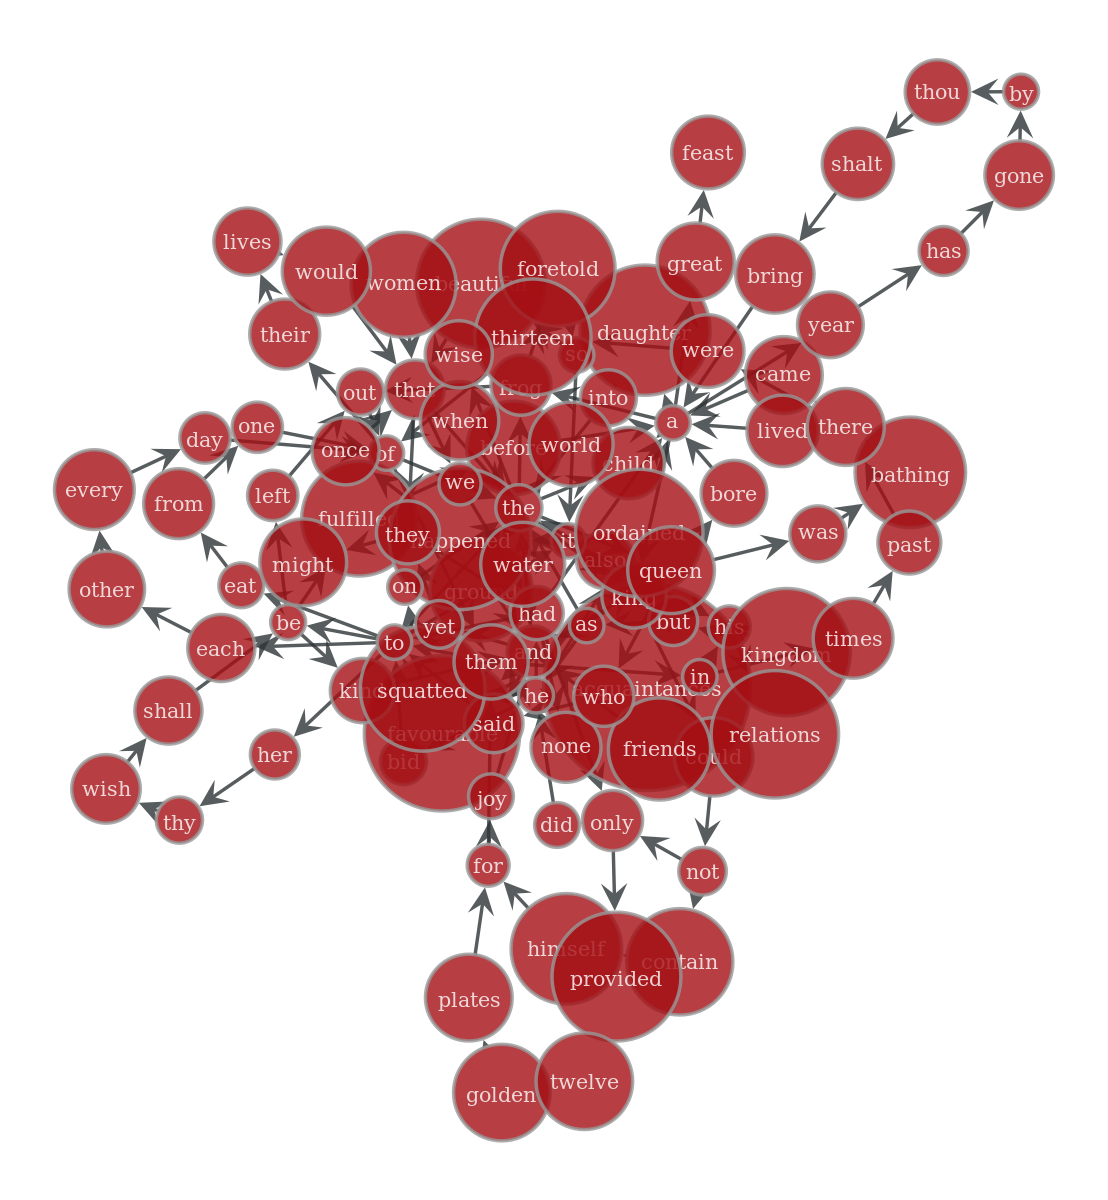
\includegraphics[scale=0.2]{englishwordgraph.png}
	\caption{}
	\label{fig:engword}
\end{subfigure}
\hfill
\begin{subfigure}{.45\textwidth}
	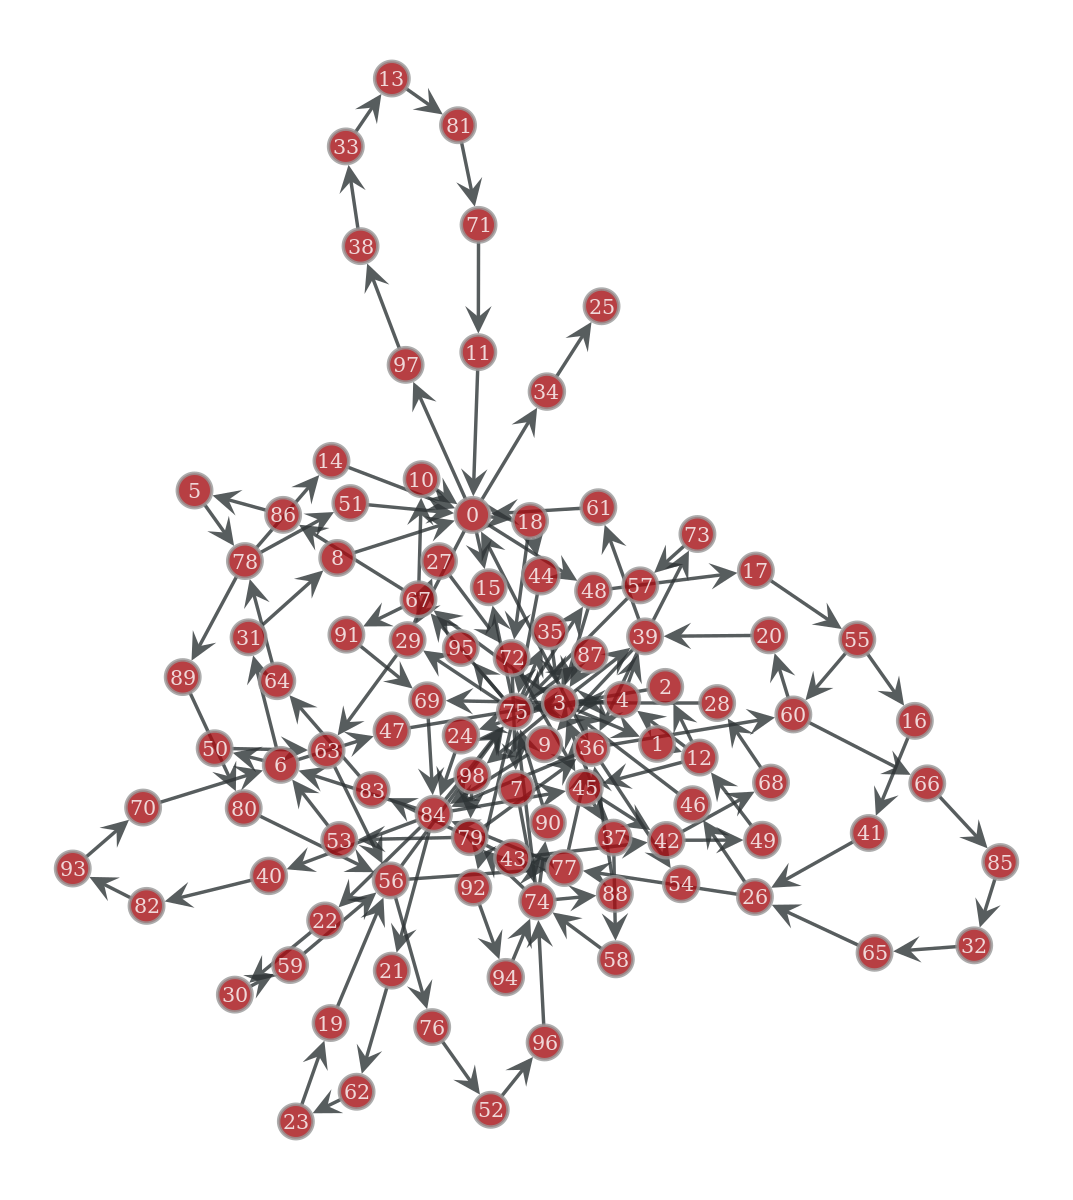
\includegraphics[scale=0.2]{englishnumbergraph.png}
	\caption{}
	\label{fig:engnum}
\end{subfigure}
\caption{Initial graphs generated off the English story corpus. (a) shows the graph with vertex labelling of their corresponding words. (b) shows the same graph but with integer labels rather than word labels to provide better visibility.}
\end{figure}

As done in the Early Experimentations of the karate club dataset, we calculate the values of the various graph properties explained in Chapter 2. These are graph properties such as local clustering coefficient, betweenness centrality, closeness centrality, trophic levels and additionally, page rank. Values are organised into their corresponding columns and presented as a table using abbreviations of each graph property. For example, ``TL" for trophic levels, ``CC" for closeness centrality, etc. The ten most frequently used words are shown in Table \ref{table:englishtop} below. Where the count denotes the frequency of the words appearance in the English story corpus. 

\begin{table}[!htb]
\centering
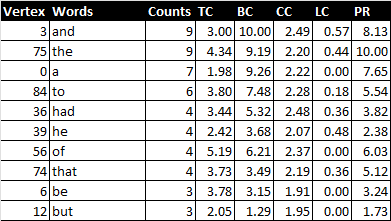
\includegraphics[scale=0.9]{englishtabletop10.png}
\caption{The first 10 most common words of the dataset. Generated from the English version of ``Sleeping Beauty" in a table format.}
\label{table:englishtop}
\end{table}

We begin by analysing words with the most recurrences (see Table \ref{table:englishtop}). In the order of most frequent to least, the words are ``and'', ``the", ``a", ``to", ``had", ``he", ``of", ``that", ``be" and ``but". Note that nouns, adverbs and adjectives do not appear in the most frequent words. These are the words that are deemed more vital in the creation of structure within a sentence of the story corpus. Any sentence in ``Sleeping Beauty" will have a high chance of containing at least one of these words. Since this is only a portion of a dataset, we can compare these words to a larger dataset to see whether or not the importance of these words remain same. Word frequencies follow the Zipf curve for languages, as discussed in the previous section, so we can take another corpus to compare its frequency of words to ours. We choose to compare the story corpus to the British National Corpus (BNC) \cite{bnc2007british} which is a 100 million word collection that includes both written and spoken English language. The benefits in choosing BNC is that it contains older English so may provide clearer correlations to the story of ``Sleeping Beauty" (the Brothers Grimm version began in the late 18th century). So for the BNC, the top ten words \cite{leech2014word} in order of frequencies are ``the", ``of", ``and", ``a", ``in", ``to", ``it", ``is", ``to" and ``was". Comparing the most frequent words in both corpora, correlations are achieved such as the repetitions of words ``the", ``to", etc. Such similarities reinforce the fact that the English language has a structured form that requires the use of these such words, as demonstrated with a much smaller corpus compared to the the BNC.

\begin{table}[!htb]
\centering
\begin{subtable}{.45\textwidth}
	\centering
	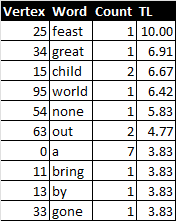
\includegraphics[scale=0.9]{engtabletctop.png}
	\caption{}
	\label{table:englishtoptc}
\end{subtable}
\hfill
\begin{subtable}{.45\textwidth}
	\centering
	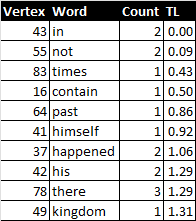
\includegraphics[scale=0.9]{engtabletcbot.png}
	\caption{}
	\label{table:englishbottc}
\end{subtable}
\caption{Partial extracts of the table data ordered by their trophic levels. (a) top 10 words and (b) bottom 10 words ranked by their trophic levels based on the English story Corpus.}
\end{table}

Now onto the analysis of Trophic levels and coherence (see Tables \ref{table:englishtoptc} and \ref{table:englishbottc}). When applying trophic level calculations on directed word graphs, the levels represent the positioning of the word within its relative sentence. Similarly shown in the analysis of network data in empirically-derived directed networks \cite{johnson2017looplessness}. For the ``Sleeping Beauty" English word graph, the lower trophic levels denotes the vertices most likely to be sentence starters and the higher levels denote the sentence enders. This is supported by the data because the top six words with largest trophic levels values (ranging from $10.00-4.77$) are all sentence enders or accompanied a sentence ender (vertex 34). Along with the bottom five being words (trophic values ranging from $0.00-0.86$) nearer the start of sentences such as ``there" and ``times" in relation to the corpus. However trophic incoherence is calculated to be $0.91$ which means that the levels in the graph can not be distinguished and are not clear. Since the $\text{trophic coherence} = 1 - \text{trophic incoherence} = 0.09$ which is due to the fact of the vast difference of sentence lengths in the corpus. Which varies from the shortest sentence of five words and the longest of forty seven words. Consequently in relation to the extract used, a clear hierarchical layout may not be provided but there remains a good layout for sentence flow. Demonstrated by further graphs with the trophic levels as the $y$-axis ranging from 0 to 10 downwards to provide a normal cascade of words. Then the $x$-axis ranging from 0 to 10 from left to right which will be based on other graphical properties.

\begin{table}[!htb]
\centering
\begin{subtable}{.2\textwidth}
	\centering
	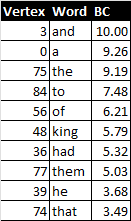
\includegraphics[scale=0.9]{englishtablebc.png}
	\caption{}
	\label{table:englishtablebc}
\end{subtable}
\hfill
\begin{subtable}{.2\textwidth}
	\centering
	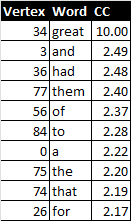
\includegraphics[scale=0.9]{englishtablecc.png}
	\caption{}
	\label{table:englishtablecc}
\end{subtable}
\hfill
\begin{subtable}{.2\textwidth}
	\centering
	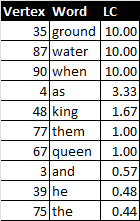
\includegraphics[scale=0.9]{englishtablelc.png}
	\caption{}
	\label{table:englishtablelc}
\end{subtable}
\hfill
\begin{subtable}{.2\textwidth}
	\centering
	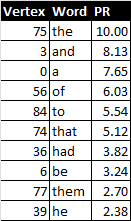
\includegraphics[scale=0.9]{englishtablepr.png}
	\caption{}
	\label{table:englishtablepr}
\end{subtable}
\caption{Partial extracts of the English table data ordered by their (a) betweenness centrality values, (b) closeness centrality values, (c) local clustering coefficients and (d) page ranks.}
\end{table}

Extraction of the top ten vertices for each graph property to provide ease of comparison later on with the graph visualisations.

\begin{figure}[!htb]
\centering
\begin{subfigure}{.45\textwidth}
	\hspace{-1.2cm} 
	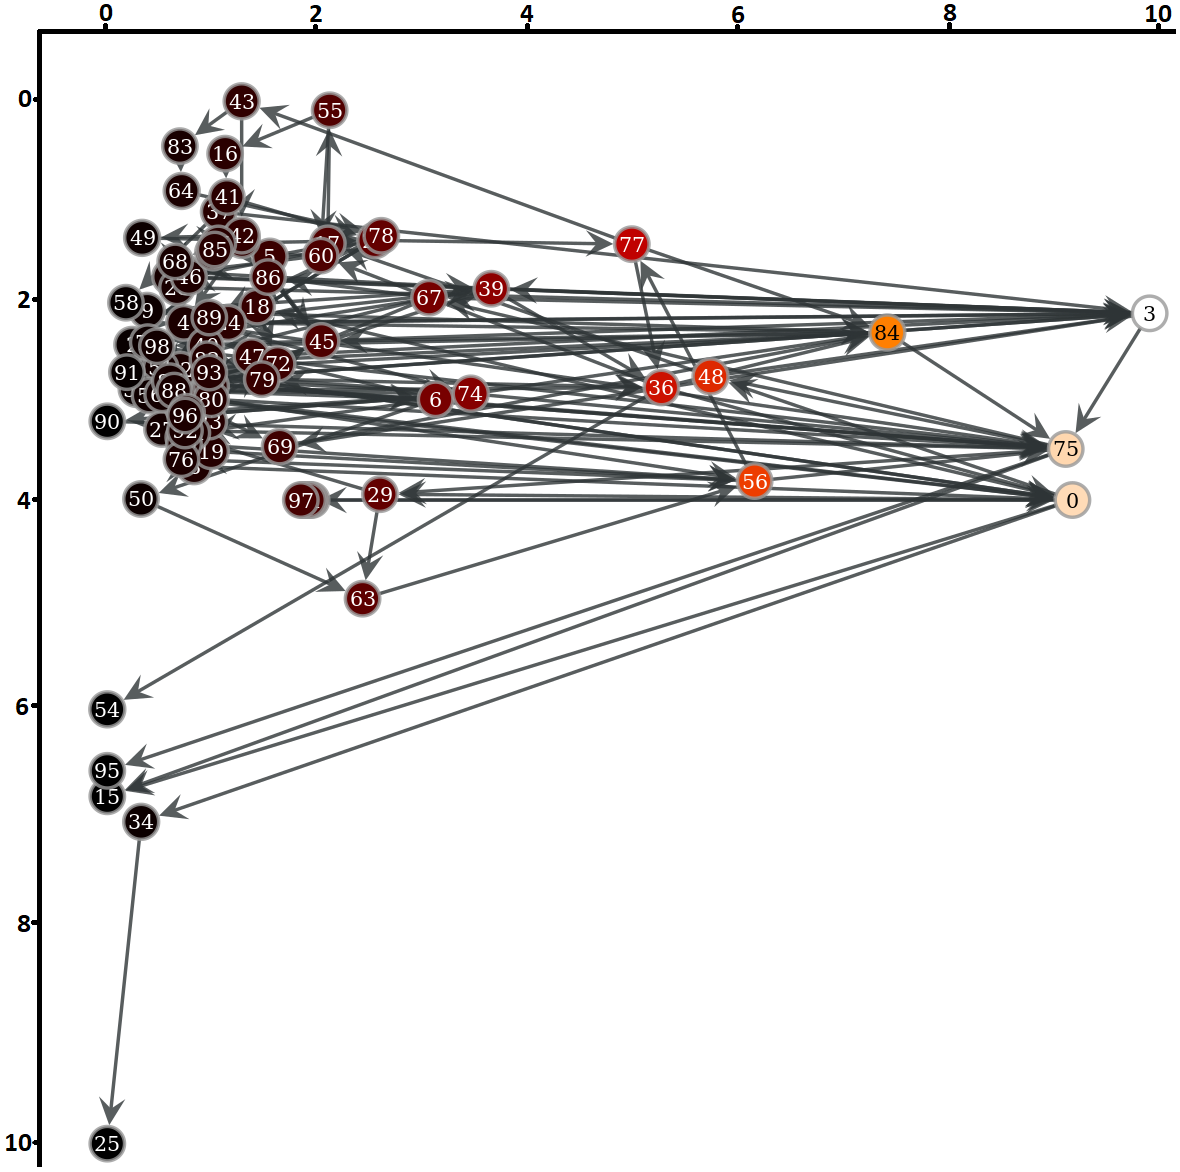
\includegraphics[scale=0.26]{englishbetweenness.png}
	\caption{}
	\label{fig:engbc}
\end{subfigure}
\hfill
\begin{subfigure}{.45\textwidth}
	\hspace{-1cm} 
	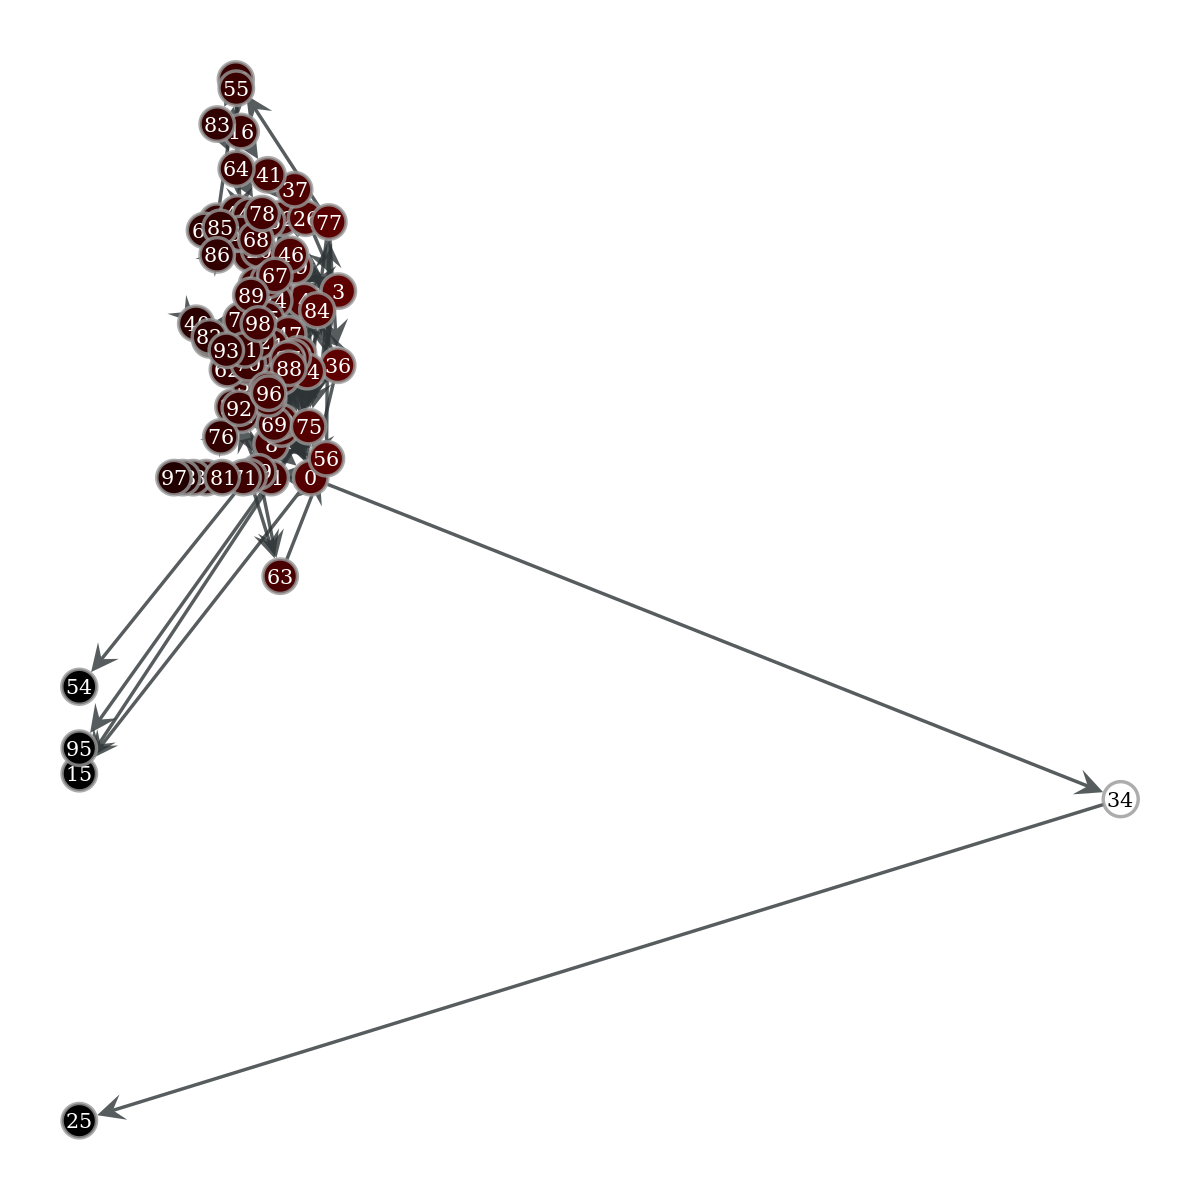
\includegraphics[scale=0.26]{englishcloseness.png}
	\caption{}
	\label{fig:engcc}
\end{subfigure}
\caption{The $x$-axis positioning of vertices are altered based on their (a) betweenness centrality and (b) closeness centrality values. The $y$-axis uses the trophic levels. Since the axis is the same for any graph, due to normalised values, further graphs will not contain the axis for clarity.}
\end{figure}

As visually demonstrated on Figures \ref{fig:engbc} and \ref{fig:engcc}, the centrality values for each word is plotted against their trophic levels. Both have been normalised to a range of 0-10 with Figure \ref{fig:engbc} showing the betweenness centrality on the x-axis and Figure \ref{fig:engcc} showing the closeness centrality. The axis are provided here to demonstrate the ranges however will not be included for future graphs because they follow the same axis layout.

Key vertices can be visually identified based on their betweenness values. These vertices are vertex 3, 0 and 75 which are the words ``and", ``a" and ``the" respectively (shown by the Table \ref{table:englishtablebc}). These are conjunctions and determiners of the English language and they have the largest frequency of appearance in the story corpus discussed before. Demonstrating a strong link between the betweenness centrality values of vertices to the word frequencies within the text. Furthermore, these words are common in forming correct structure of a typical English sentence meaning that high betweenness associates the words as key bridges in a sentence. 

When considering closeness centrality, the graph shows that almost all vertices have a similar closeness value in comparison to their betweenness. This is because the closeness centrality analyses the importance of the words within their local clusters rather than the graph as a whole. Meaning that words with high closeness values are key connections in their relative clusters, in other words the sentences that they are part of. However vertex 34 (the word ``great") is an outlier and by further analysis, vertex 34 is the only connection between vertex 0 and 25. Also vertex 25 has the highest trophic level and vertex 0 has a low trophic level but a higher degree. Consequently, the closeness value for 34 is an extreme due to the fact that it is the only predecessor of vertex 25. Thus meaning that vertex 34 is the only local bridge in its sentence giving it an extreme closeness whereas other vertices contains multiple connections.

In conclusion, based on the story corpus, betweenness finds the words most commonly used as connectors in a sentence and closeness finds the words that are likely to isolate later vertices.

\begin{figure}[!htb]
\centering
\begin{subfigure}{.45\textwidth}
	\hspace{-1cm} 
	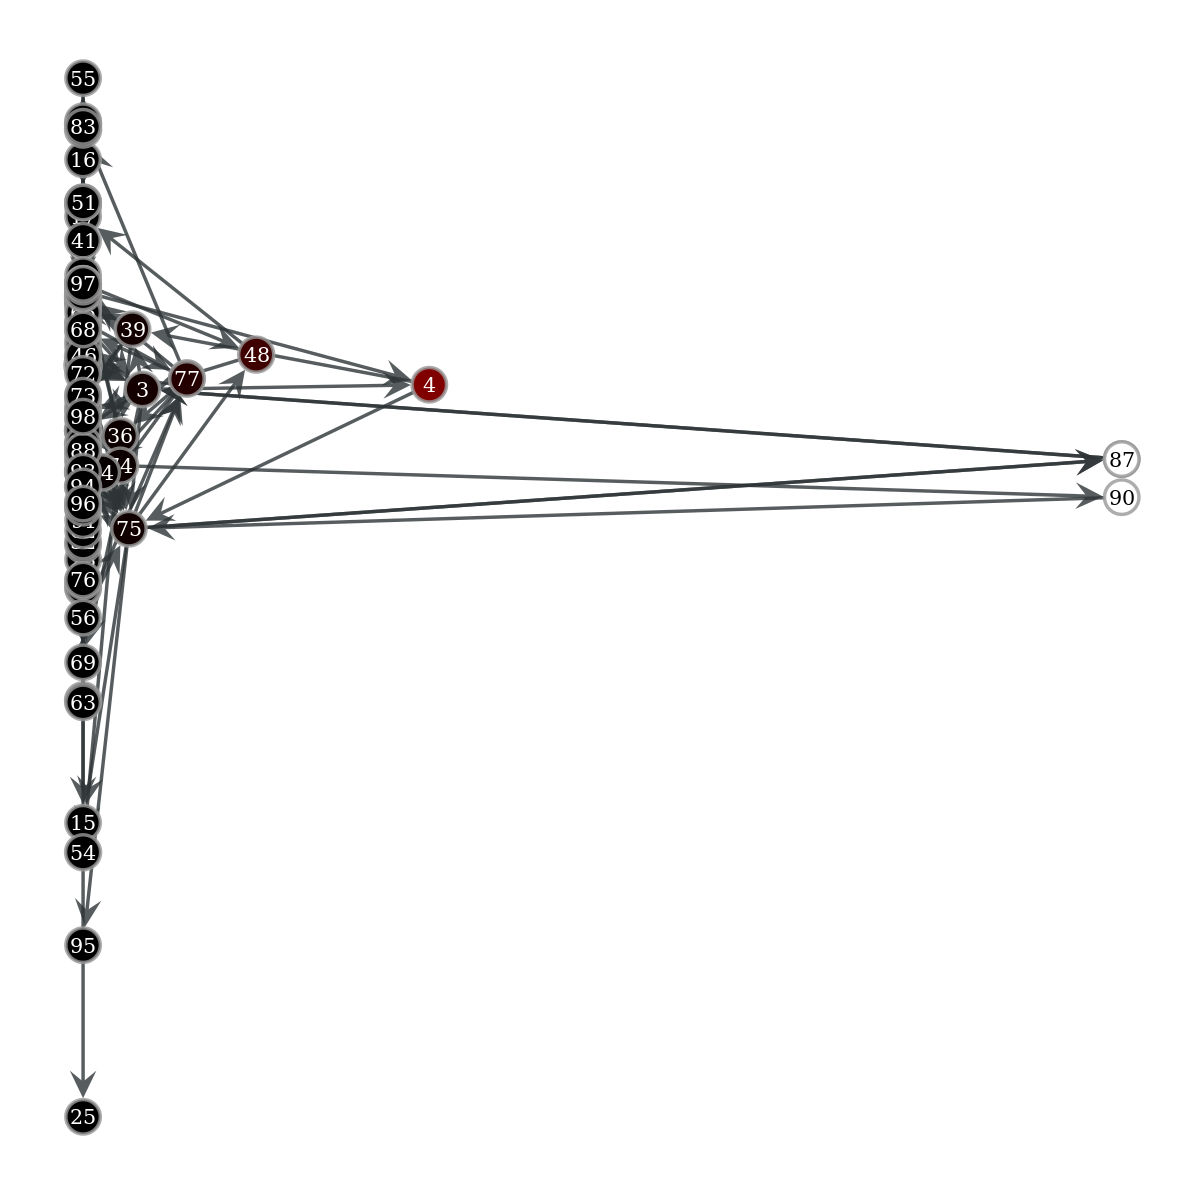
\includegraphics[scale=0.2]{englishlocalclustering.png}
	\caption{}
	\label{fig:englc}
\end{subfigure}
\hfill
\begin{subfigure}{.45\textwidth}
	\hspace{-1cm} 
	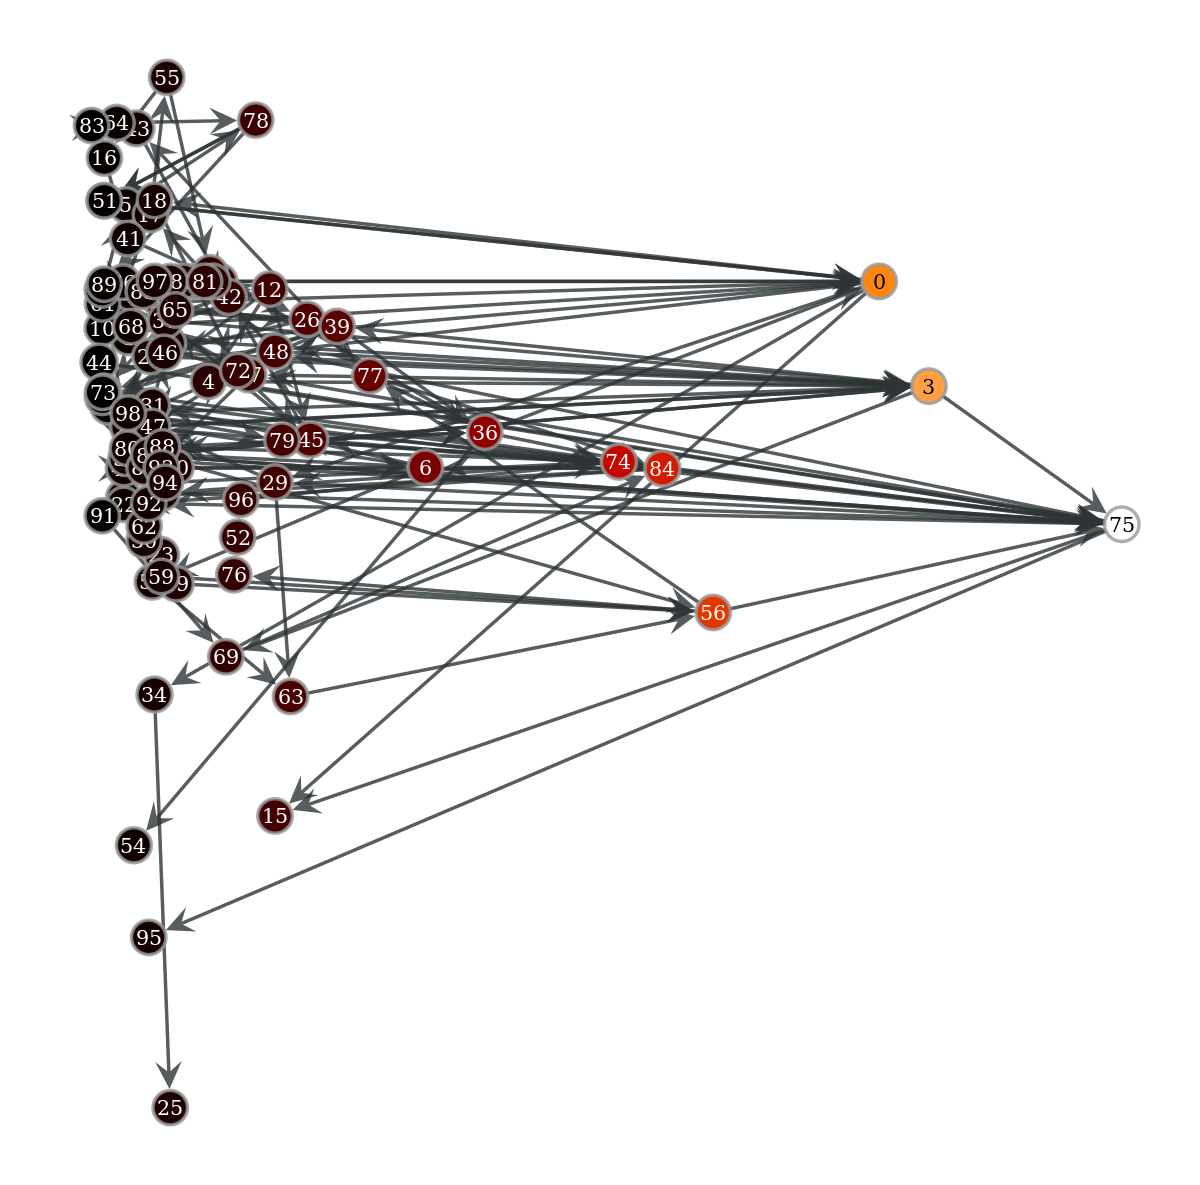
\includegraphics[scale=0.2]{englishpagerank.png}
	\caption{}
	\label{fig:engpr}
\end{subfigure}
\caption{Instead of centrality values like before, (a) local clustering coefficients and (b) page ranks are used for the $x$-axis. The $y$ values remains the same representing the trophic levels.}
\end{figure}

Finally, local clustering coefficients and page ranks of the vertices within the English word graph are presented similarly as before.  Local clustering coefficients in Figure \ref{fig:englc} and page ranks in Figure \ref{fig:engpr} along with their respective table extracts shown before in Tables \ref{table:englishtablelc} and \ref{table:englishtablepr}. 

Immediately, the local clustering graph shows very few vertices who has a high local clustering, the main ones being vertices 87 and 90 (``water" and ``when" respectively). However, there does not exist a clear relationship between these words other than neighbours of these words have have a high degree or importance in the graph. Important words such as ``and" and ``a". On the other hand this is only for the English version of the story so other languages may lead to different results. The page rank of each vertex shows the importance of each word beyond their direct contact. Essentially it has elements of both closeness and betweenness centrality which the graph reinforces since it is visually similar to the betweenness English graph.

In conclusion, when analysing the English language, trophic levels have provided a naturally flow of data presentation from top to bottom in the various graphs generated. Where some sections of the graph are grammatically correct when following their flows. Betweenness centrality and page rank both identified the words of most importance with respects to their neighbours. Closeness centrality also identified words of key importance but at a local level. Finally local clustering coefficients do not provide sufficient benefits when visualising the dataset in the English language. Therefore the results generated based on the English version can be extrapolated to represent the English language. Which is achieved through the identification of the words position in the structure of a sentence and its relative importance. This could also be used for languages that have a similar grammatical structure to English. Now we move onto the analysis of a different translation of the story corpus, German.

\subsection{German}
German is also a Germanic language under the Indo-European language family, same as English. However whilst modern English no longer uses the inflectional case system in grammar, the German language still does \cite{durrell2011hammer}. So as well as the parts of speech in English, German words can be divided into two groups, the words which are \emph{inflectable} and \emph{uninflectable}. If a word is inflectable then their form changes based on the context that the word is used in. These include the three genders for the words (masculine, feminine and neutral), the four cases (nominative, accusative, genitive and dative) and the number (singular or plural). Uninflectable words are known as \emph{modal particles} and mainly used to highlight an emotion of the sentence in spoken language. Therefore the German language is considerably more varied compared to the English language. Meaning that, in theory, the dataset would contain more unique words overall. Which is proven to be true as the dataset based on the story corpus for German contains 109 words whilst English had only 99.

Expectations of the graph properties for the German language is that there would be more unique words of higher importance based on the different genders for words and particles. Word graphs for the German version of the story corpus are generated and shown in Figure \ref{fig:gergraph}. Similarly as before, each number references the same word in its position.

\begin{figure}[!htb]
\centering
\begin{subfigure}{.45\textwidth}
	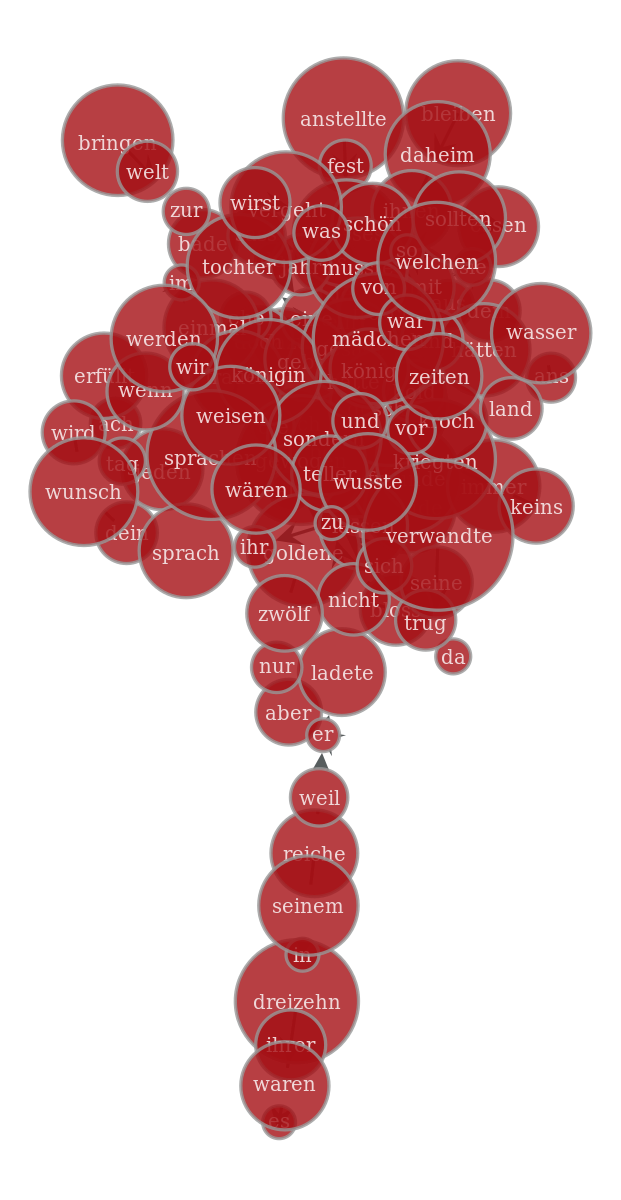
\includegraphics[scale=0.2]{germanwordgraph.png}
	\caption{}
	\label{fig:gerword}
\end{subfigure}
\hfill
\begin{subfigure}{.45\textwidth}
	\hspace{-2cm} 
	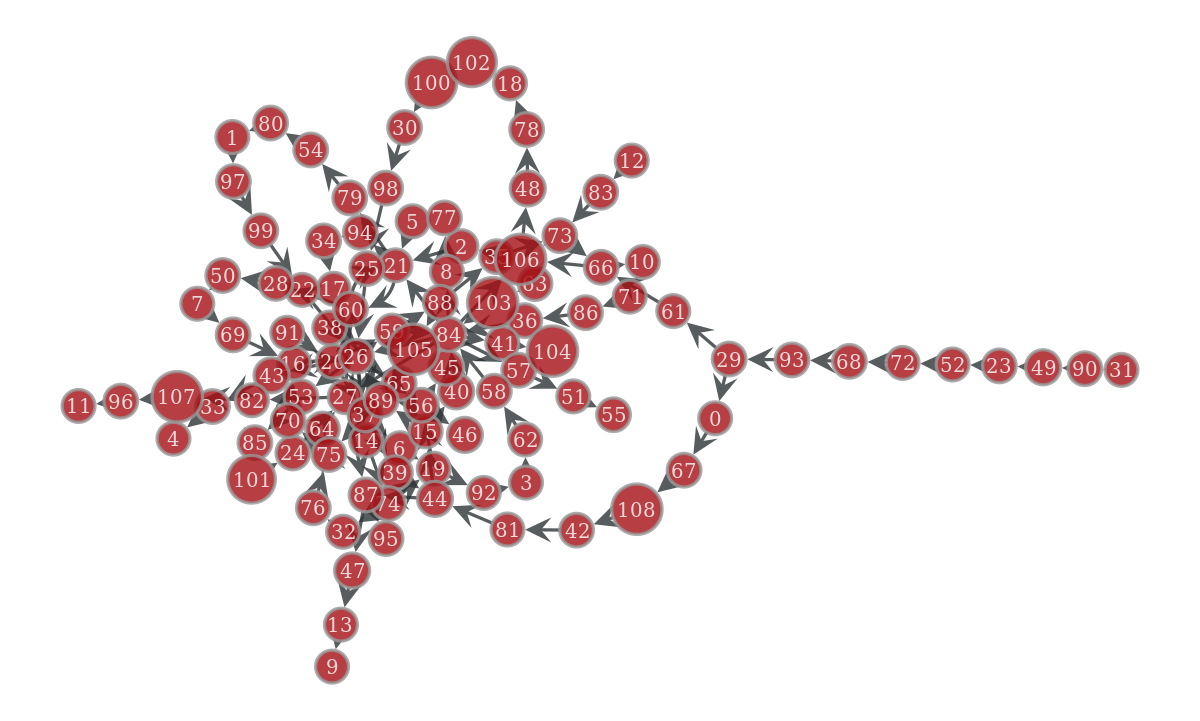
\includegraphics[scale=0.2]{germanwordgraphnumbered.png}
	\caption{}
	\label{fig:gernum}
\end{subfigure}
\caption{The German (a) word graph and (b) numbered equivalent of the word graph generated from the German translation of the ``Sleeping Beauty" corpus.}
\label{fig:gergraph}
\end{figure}

\begin{table}[!htb]
\centering
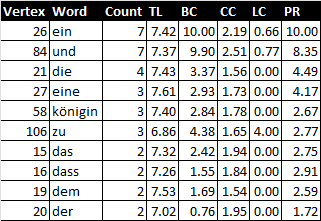
\includegraphics[scale=0.9]{germantabletop10.png}
\caption{Top 10 words with the highest frequency in the German dataset including values of other graph properties. }
\label{table:germantop}
\end{table}

Table \ref{table:germantop} shows the most common ten words in the German dataset along with each graph property value. The translation to English for each word in the order of the table is ``and", ``a" (Masculine), ``the" (Feminine), ``to", ``a" (Feminine), ``Queen", ``King", ``not", ``himself/herself/itself" (dependent on the pronoun this refers to) and ``the" (Neutral). As expected when comparing to the English dataset most words appear in both translations as the top ten, in particular the top three. Which we recall was ``and", ``the" and ``a" for the English dataset. However rather than a cumulative count of ``the" in English, the German translation has multiple versions. This may counteract each others importance and bring they values lower. By retaining the inflectable changes in grammar, the average count is lower for the German translation. Additionally the range of frequencies has also decreased from 9-1 to 7-1. For example, ``the" in English was split into ``die", ``der" and ``das" in German. By noting these key differences, the graphical properties will be analysed.

\begin{table}[!htb]
\centering
\begin{subtable}{.45\textwidth}
	\centering
	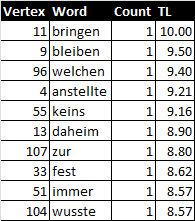
\includegraphics[scale=0.9]{gertabletctop.png}
	\caption{}
	\label{table:germantoptc}
\end{subtable}
\hfill
\begin{subtable}{.45\textwidth}
	\centering
	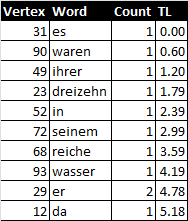
\includegraphics[scale=0.9]{gertabletcbot.png}
	\caption{}
	\label{table:germanbottc}
\end{subtable}
\caption{Tables for (a) top 10 and (b) bottom 10 trophic levels of the German dataset along with other graph values.}
\end{table}

Analysis of the trophic levels demonstrates that most words congregate at around $7.3$. This can be more evidently seen in the graphical representations on Figures \ref{fig:gercentrality} and \ref{fig:gerother} later on. From the same graphs, there is a unique path from vertex 31 to 29 which is equivalent to the translation ``Es waren ihrer dreizehn in seinem Reiche, weil er". This path is grammatically correct and represents the beginning of a sentence belonging to the German story corpus. Furthermore this portion holds only unique words, hence has not been influenced by other vertices so demonstrates a clear hierarchical structure. Which is the reason the words used are of low trophic levels. Whereas most other sentences share words which causes the conglomeration nearer $7.3$. Consequently the German language has more options for word choices which means the increased probability of unique sentences.

Trophic coherence has also benefited from the uniqueness of word choices since for the German graph, trophic coherence is calculated to be $0.29$. This is larger than the English graph which was $0.09$. Therefore the German graph has a clearer hierarchical structure compared to the English graph with clearer levels as demonstrated in further graphs below when analysing other properties.

\begin{table}[!htb]
\centering
\begin{subtable}{.2\textwidth}
	\centering
	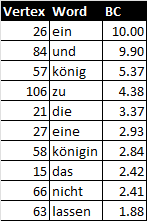
\includegraphics[scale=0.9]{germantablebc.png}
	\caption{}
	\label{table:germantablebc}
\end{subtable}
\hfill
\begin{subtable}{.2\textwidth}
	\centering
	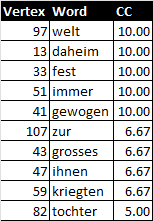
\includegraphics[scale=0.9]{germantablecc.png}
	\caption{}
	\label{table:germantablecc}
\end{subtable}
\hfill
\begin{subtable}{.2\textwidth}
	\centering
	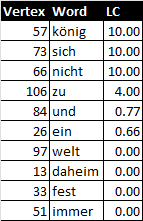
\includegraphics[scale=0.9]{germantablelc.png}
	\caption{}
	\label{table:germantablelc}
\end{subtable}
\hfill
\begin{subtable}{.2\textwidth}
	\centering
	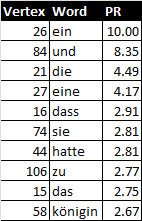
\includegraphics[scale=0.9]{germantablepr.png}
	\caption{}
	\label{table:germantablepr}
\end{subtable}
\caption{Partial extracts of the German table data ordered by their (a) betweenness centrality values, (b) closeness centrality values, (c) local clustering coefficients and (d) page ranks.}
\label{table:germandata}
\end{table}

Entirety of the data presented in table form can be seen in Appendix \ref{app:}. Table \ref{table:germandata} (a)-(d) shows an extract of the top 10 complex values in order of highest to lowest for each property.

\begin{figure}[!htb]
\centering
\begin{subfigure}{.45\textwidth}
	\hspace{-1cm} 
	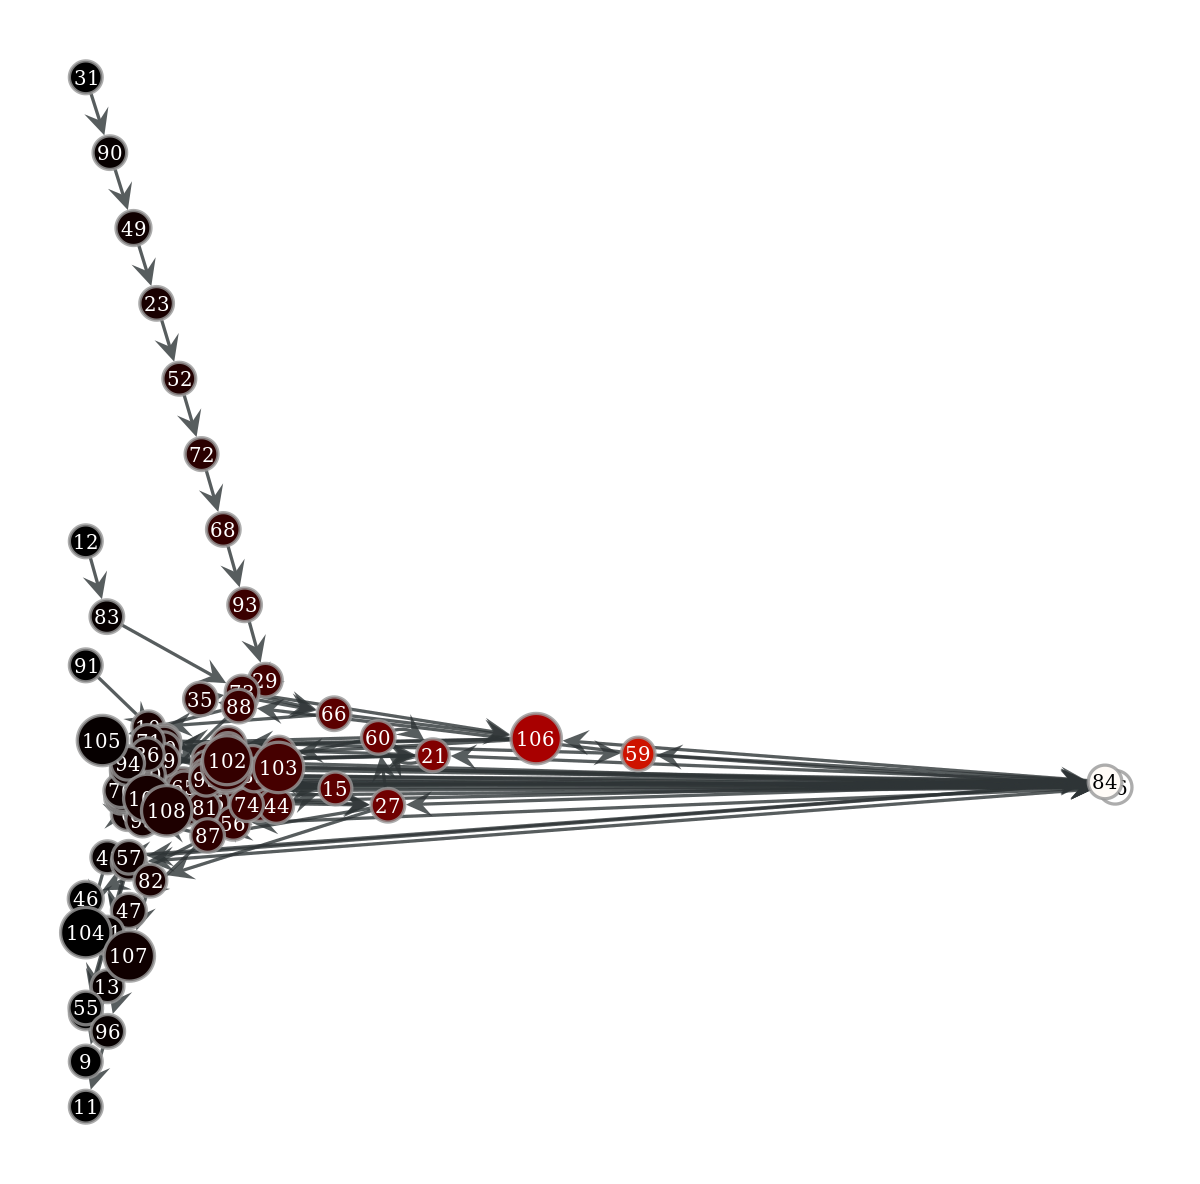
\includegraphics[scale=0.2]{germanbetweenness.png}
	\caption{}
	\label{fig:gerbc}
\end{subfigure}
\hfill
\begin{subfigure}{.45\textwidth}
	\hspace{-1cm} 
	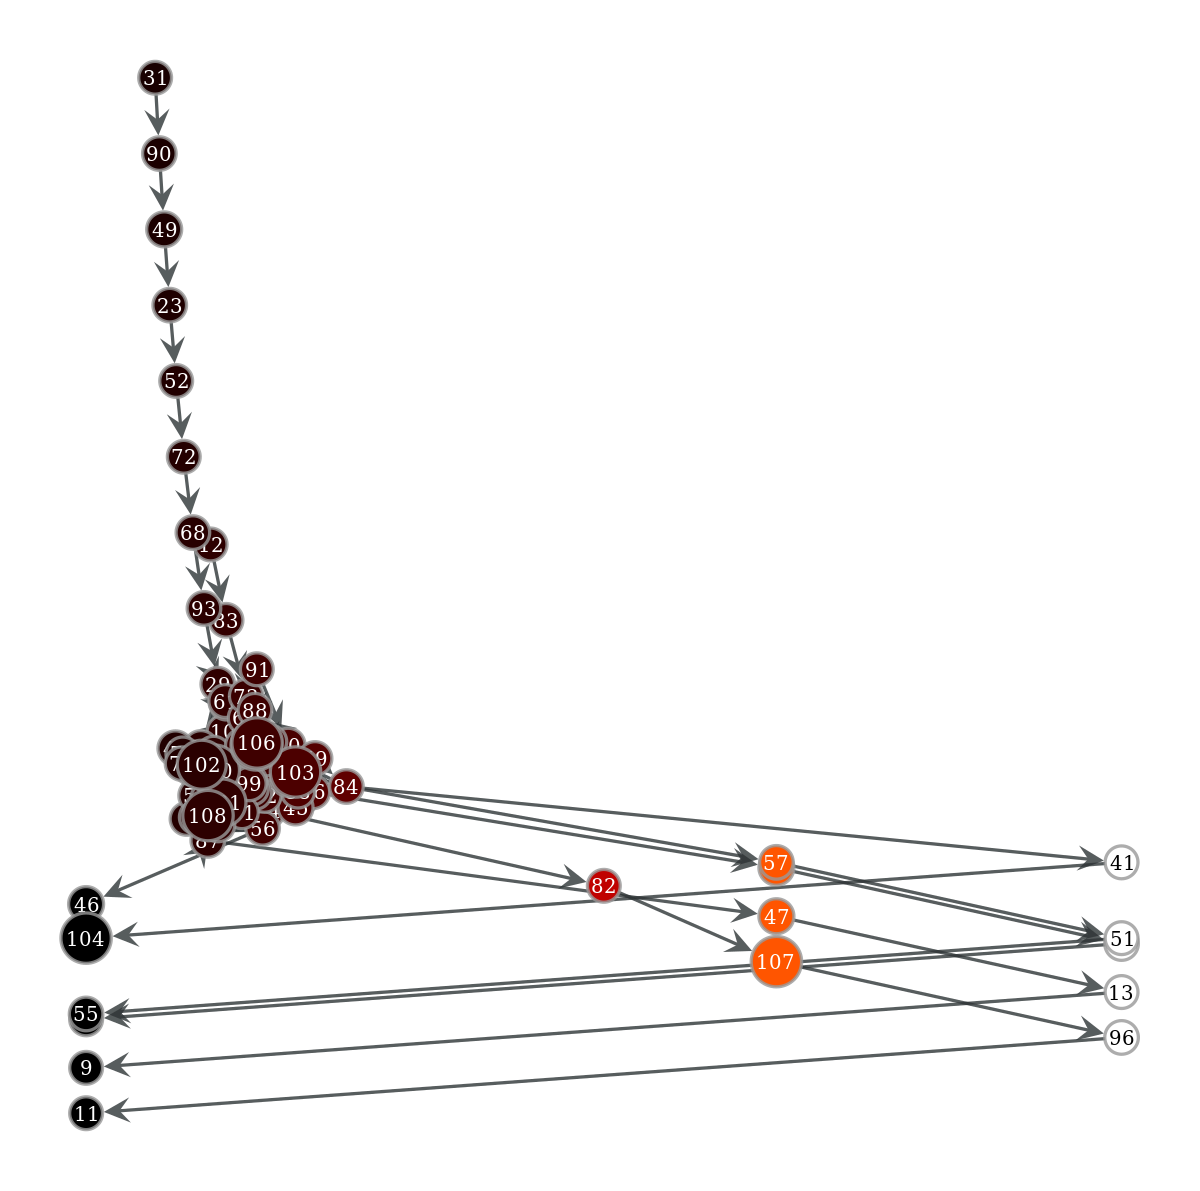
\includegraphics[scale=0.2]{germancloseness.png}
	\caption{ }
	\label{fig:gercc}
\end{subfigure}
\caption{Graphs with the $x$ positioning based on (a) betweenness and (b) closeness centrality. The $y$ is based on trophic levels.}
\label{fig:gercentrality}
\end{figure}

Assessing the visual graphs (Figures \ref{fig:gerbc} and \ref{fig:gercc}), we identify vertex 84 and 26 who have the highest betweenness  values. A correlation to the frequencies of the words in the German Story Corpus can be seen through these vertices. Additionally, the same correlation was also true in the English version because the vertices in both versions referred to the words that are most commonly used as bridges or links in sentences. In the German case, the words are ``ein" and ``und".

With closeness centrality, it is a measure of influence on nearby words, the graph in Figure \ref{fig:gercc} shows that the vertices 97, 13, 33, 51 and 41 have the largest closeness values. These all correspond to the second to last word of each sentence apart from the first sentence which has the word ``Kind" as the second to last word. However ``Kind" is also used elsewhere meaning that its closeness value was influenced through other connections. The vertices of high closeness are unique and essential as a bridge in its nearby words. Otherwise the neighbours of these vertices are likely to be isolated. Note that the orange vertices in Figure \ref{fig:gercc} are the unique words predecessors to the vertices of high closeness and the last word of every sentence always has a value of $0$.

Therefore betweenness identifies the words of key importance that are used most commonly as connectors. Meanwhile closeness identifies the words most likely to isolate vertices of the graph when following the sentence flow, i.e., breaks up the rest of the sentence into unique words. Observe that the same pattern was seen in the English version but was set aside due to there being only one vertex of high closeness. However the German version shows a correlation of local importance to unique words which means that the English version may contain the same correlation.

\begin{figure}[!htb]
\centering
\begin{subfigure}{.45\textwidth}
	\hspace{-1cm} 
	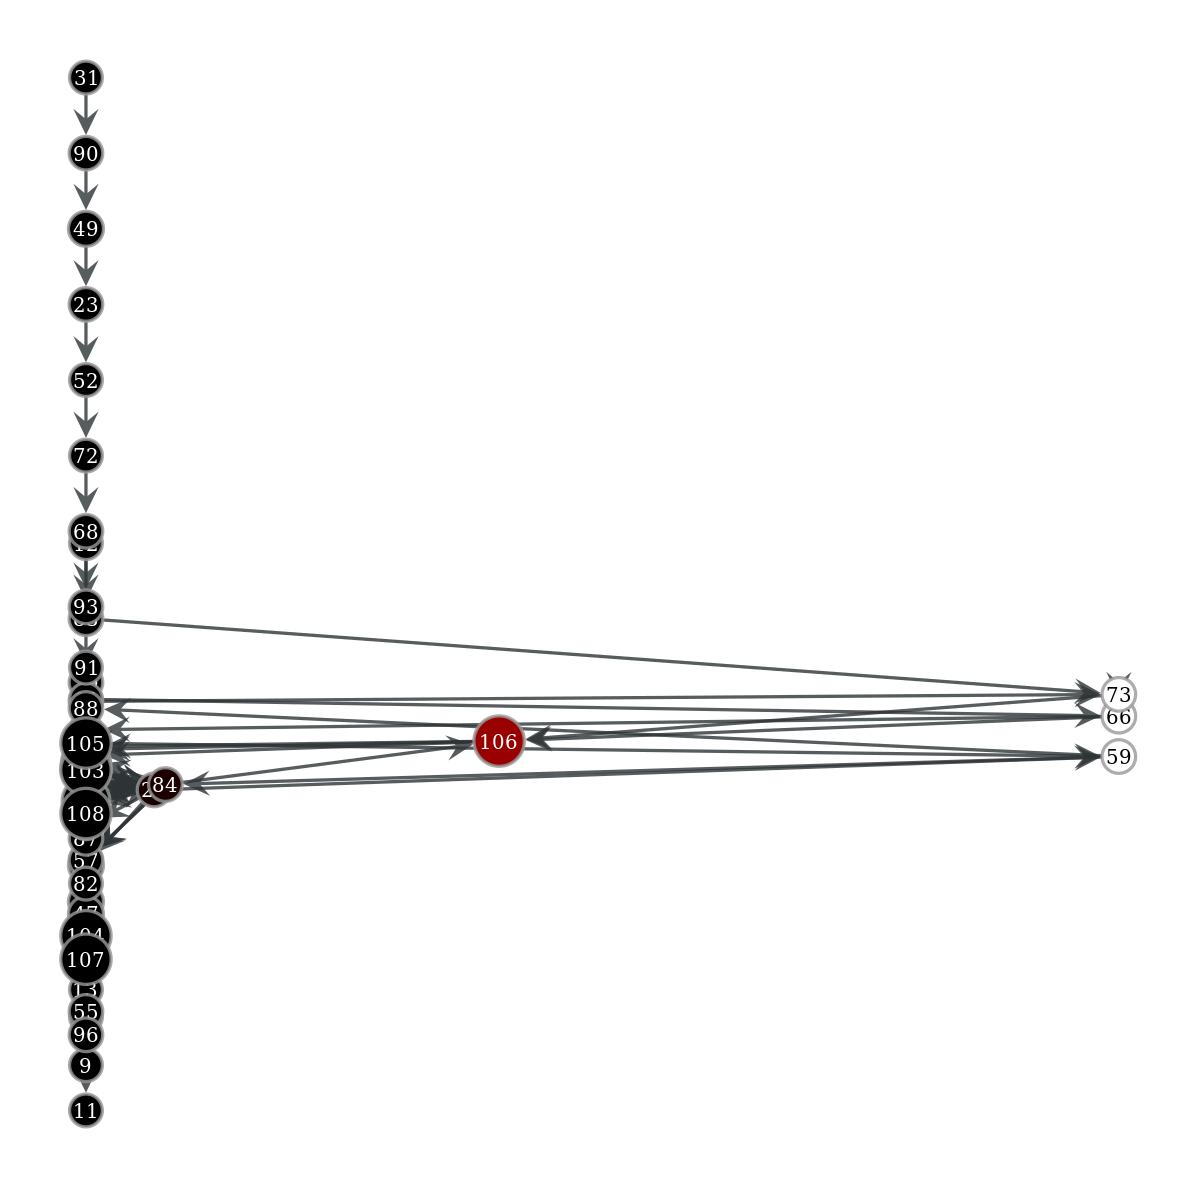
\includegraphics[scale=0.2]{germanlocalclustering.png}
	\caption{}
	\label{fig:gerlc}
\end{subfigure}
\hfill
\begin{subfigure}{.45\textwidth}
	\hspace{-1cm} 
	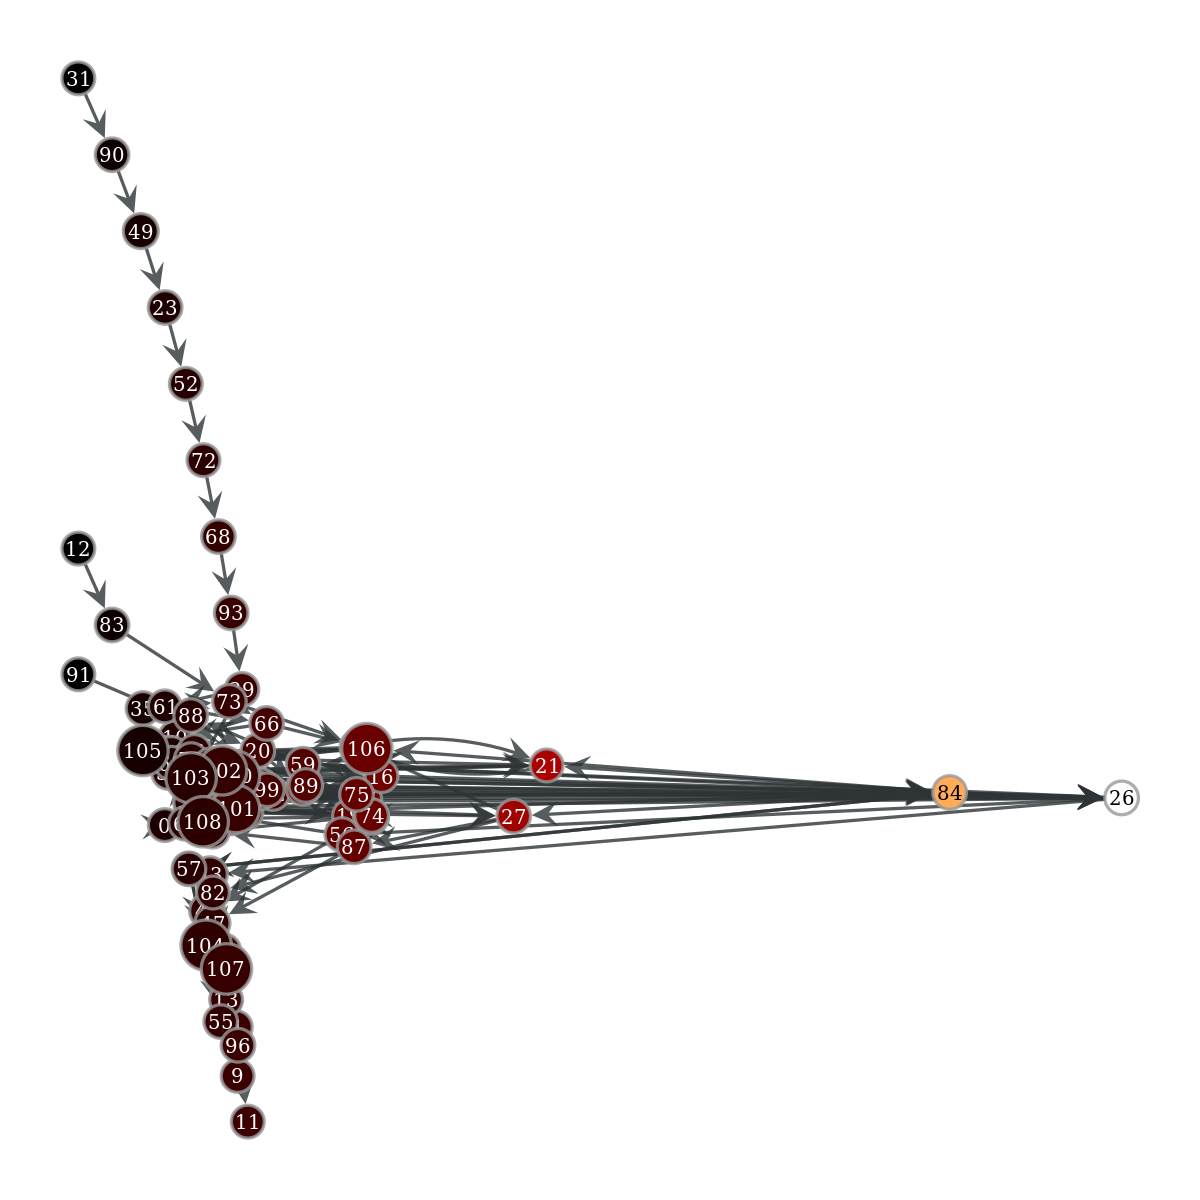
\includegraphics[scale=0.2]{germanpagerank.png}
	\caption{}
	\label{fig:gerpr}
\end{subfigure}
\caption{Displays the (a) local clustering and (b) page rank on the $x$-axis instead of the centrality values. The trophic levels for $y$ remains the same.}
\label{fig:gerother}
\end{figure}

Nothing prominent can be derived by studying the local clustering coefficients (see Figure \ref{fig:gerlc}) because almost all vertices hold a local clustering coefficient of 0 apart from six vertices. Three of which are the vertices 57, 73 and 66 which corresponds to the words ``könig", ``sich" and ``nicht" respectively. These are not unique words in the German story corpus and no other vertices demonstrate anything unique with its local coefficient. 
On the other hand, vertices with a high page rank (see Figure \ref{fig:gerpr}) correlate to either conjunctions, vertex 84 (``und"), or words that accompany other words like pronouns or articles, vertices 26 (``ein"), 27 (``eine"), etc. Therefore high page rank relates to key words that are used frequently in German, which remains true when extended to the German language as a whole.

In conclusion, similar results were seen when analysing the graphical properties based on the German and English translations. With German having a clearer visualisation and stronger correlation compared to the English language due the the uniqueness of inflectional words.

\subsection{French}
English and German are Germanic languages under the Indo-European family. Instead of another Germanic language, we study a different branch under the Indo-European family. The language being French which lies under the Italic branch of the same family. Similarly to German, French contains the same parts of speech as English but also inflectional words. So words can be inflected by number (singular or plural), gender, person, case, aspect and mood. However whilst German has three genders (Masculine, Feminine and Neutral), French \cite{hawkins2015french} only uses two, masculine and feminine. 

The story corpus is translated into the French version so graphs can be generated off this. Where the initial word graphs are shown in Figure \ref{fig:fregraph}. 

\begin{figure}[!htb]
\centering
\begin{subfigure}{.45\textwidth}
	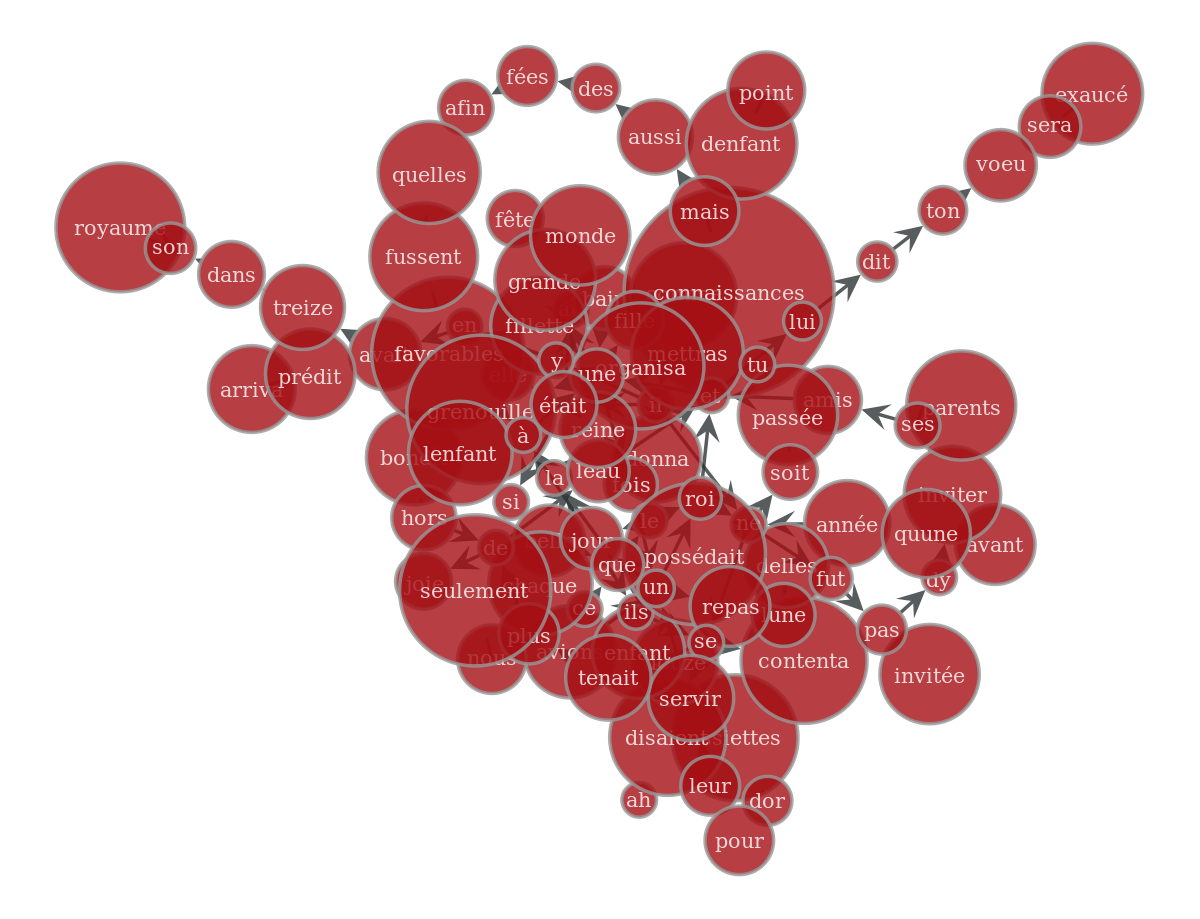
\includegraphics[scale=0.2]{frenchwordgraph.png}
	\caption{}
	\label{fig:freword}
\end{subfigure}
\hfill
\begin{subfigure}{.45\textwidth}
	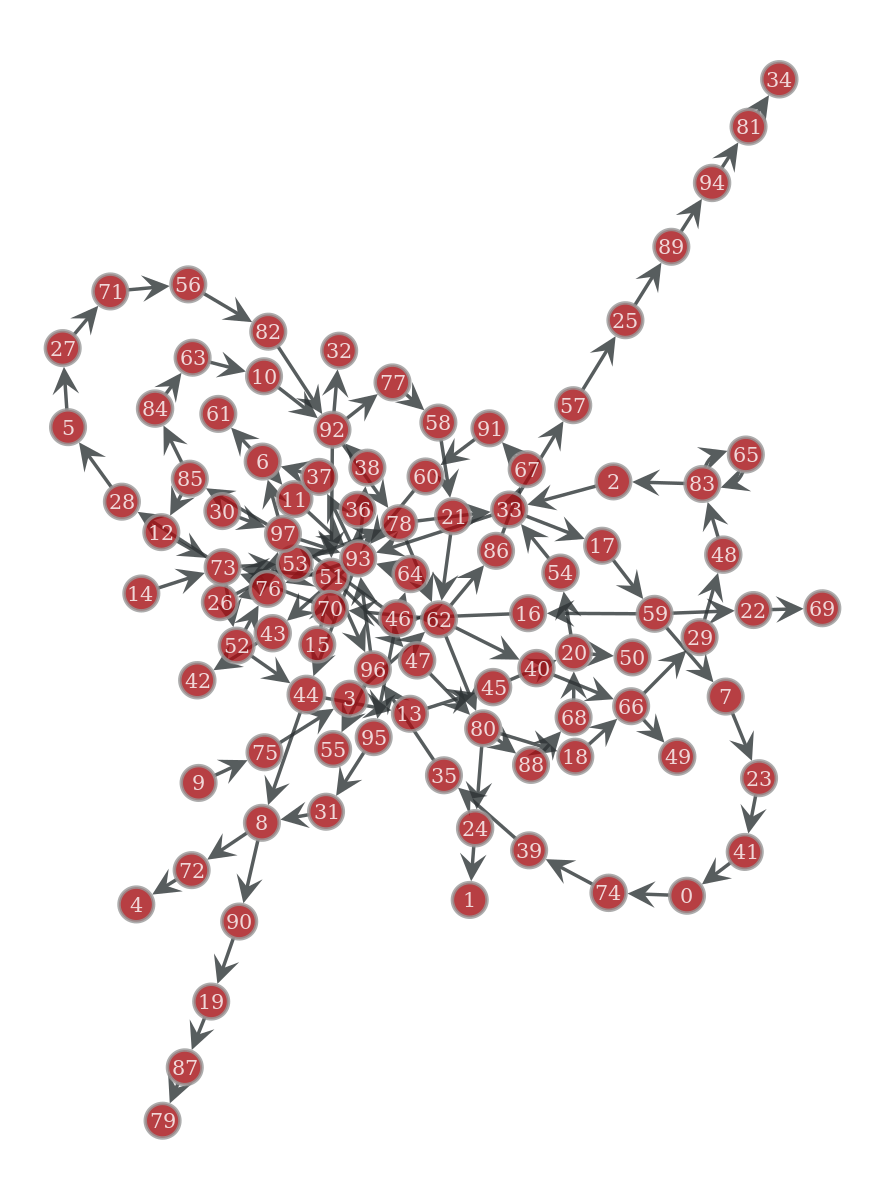
\includegraphics[scale=0.2]{frenchwordgraphnumbered.png}
	\caption{}
	\label{fig:frenum}
\end{subfigure}
\caption{The French (a) word graph and (b) numbered equivalent of the word graph generated from the French translation of the ``Sleeping Beauty" corpus.}
\label{fig:fregraph}
\end{figure}

\begin{table}[!htb]
\centering
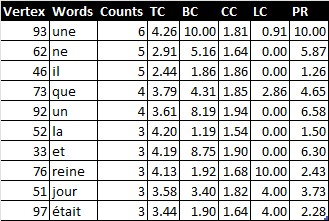
\includegraphics[scale=0.9]{frenchtabletop10.png}
\caption{Top 10 words with the highest frequency in the French translation of the corpus. Shown in table format with other graphical properties. }
\label{table:frenchtop}
\end{table}

Words of highest frequency are shown in the extract Table \ref{table:frenchtop} where the majority of words seen are inflectable and used as a way to give more information. Such as the particle of vertex 93 meaning ``a/an" or vertex 46 meaning ``he/it". So these would be used more frequently and it is generally true for the French language.

\begin{table}[!htb]
\centering
\begin{subtable}{.45\textwidth}
	\centering
	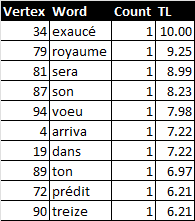
\includegraphics[scale=0.9]{frenchtabletctop.png}
	\caption{}
	\label{table:frenchtoptc}
\end{subtable}
\hfill
\begin{subtable}{.45\textwidth}
	\centering
	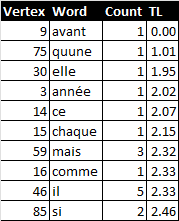
\includegraphics[scale=0.9]{frenchtabletcbot.png}
	\caption{}
	\label{table:frenchbottc}
\end{subtable}
\caption{Trophic levels, (a) top 10 and (b) bottom 10 in table format including other values.}
\end{table}

In relation to the story corpus, French has a high trophic coherence which is calculated to be $0.36$ which is higher than both English and German. Even though it may not be close to $1$, in comparison to previous languages, a clearer level structure can be identified for the French language. Top 10 trophic levels can be seen in Table \ref{table:frenchtoptc} where the high values represent the words nearer to the end of a sentence. All top 10 are within the last four words of sentences in the story corpus. However the predecessors of the words have an impact on their trophic level. If the predecessors of a word is involved in other sentences at a earlier stage then the predecessors trophic value will be lowered. Subsequently lowering the trophic levels of the neighbourhood of the word. This can be seen by vertex 49 who has a trophic level of $5.08$ even though it is last in its sentence.

\begin{table}[!htb]
\centering
\begin{subtable}{.27\textwidth}
	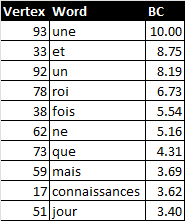
\includegraphics[scale=0.9]{frenchtablebc.png}
	\caption{}
	\label{table:frenchtablebc}
\end{subtable}
\hfill
\begin{subtable}{.2\textwidth}
	\centering
	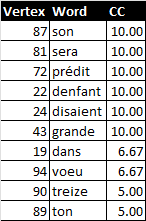
\includegraphics[scale=0.9]{frenchtablecc.png}
	\caption{}
	\label{table:frenchtablecc}
\end{subtable}
\hfill
\begin{subtable}{.2\textwidth}
	\centering
	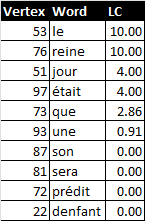
\includegraphics[scale=0.9]{frenchtablelc.png}
	\caption{}
	\label{table:frenchtablelc}
\end{subtable}
\hfill
\begin{subtable}{.2\textwidth}
	\centering
	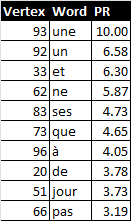
\includegraphics[scale=0.9]{frenchtablepr.png}
	\caption{}
	\label{table:frenchtablepr}
\end{subtable}
\caption{Partial extracts of the French table data ordered by their (a) betweenness centrality values, (b) closeness centrality values, (c) local clustering coefficients and (d) page ranks.}
\label{table:frenchdata}
\end{table}

Tables \ref{table:frenchdata} (a)-(d) shows an top 10 extract of Table \ref{app:} in the order of their corresponding graph property value.

\begin{figure}[!htb]
\centering
\begin{subfigure}{.45\textwidth}
	\hspace{-1cm} 
	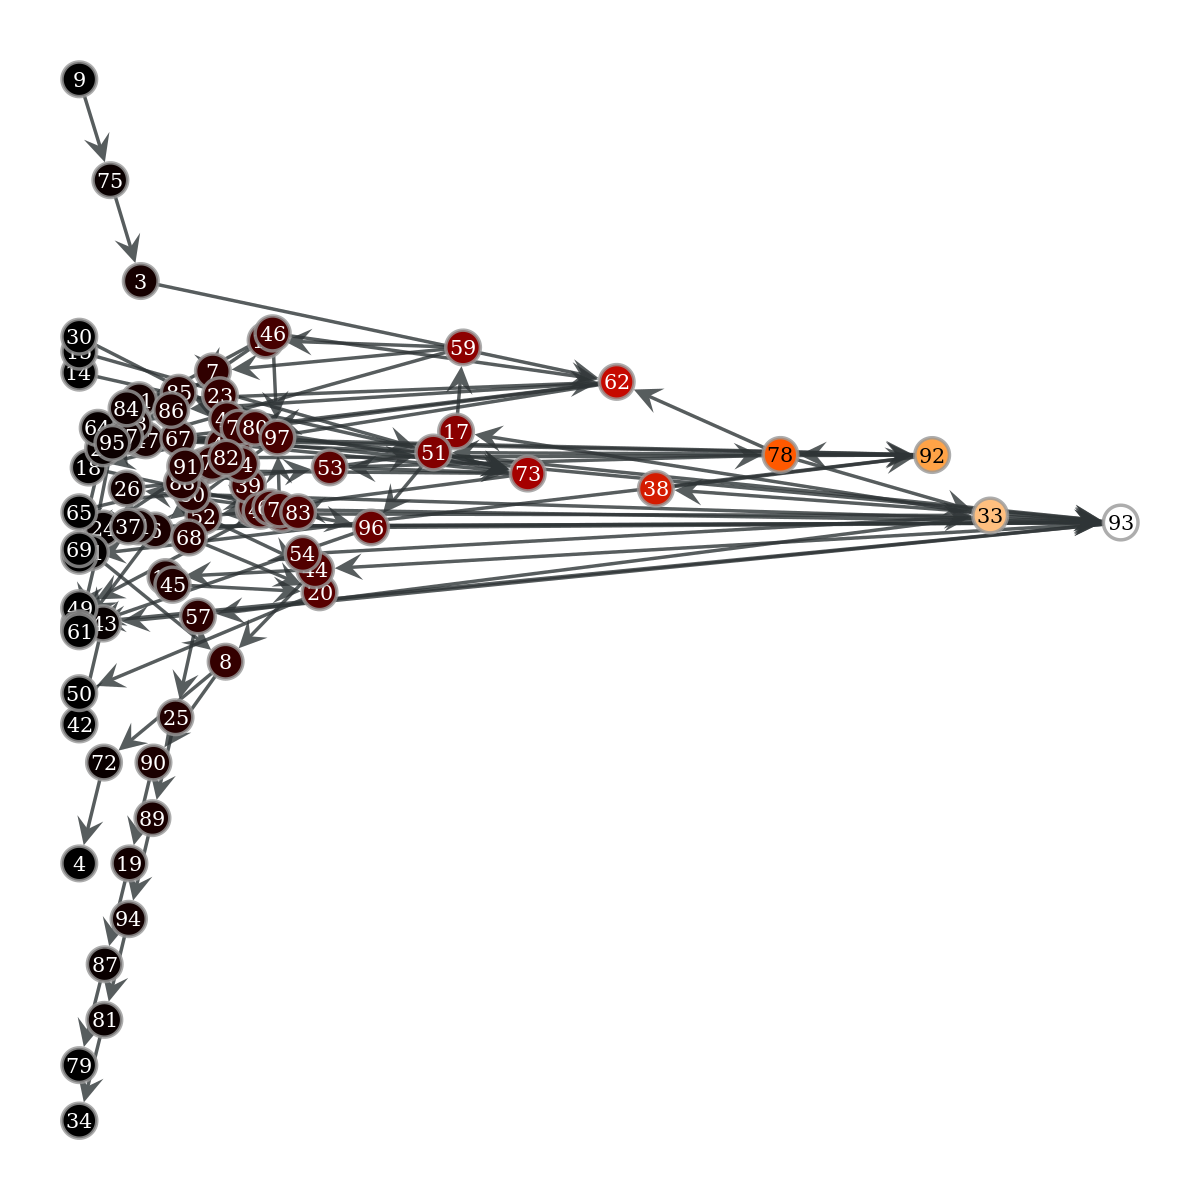
\includegraphics[scale=0.2]{frenchbetweenness.png}
	\caption{}
	\label{fig:frbc}
\end{subfigure}
\hfill
\begin{subfigure}{.45\textwidth}
	\hspace{-1cm} 
	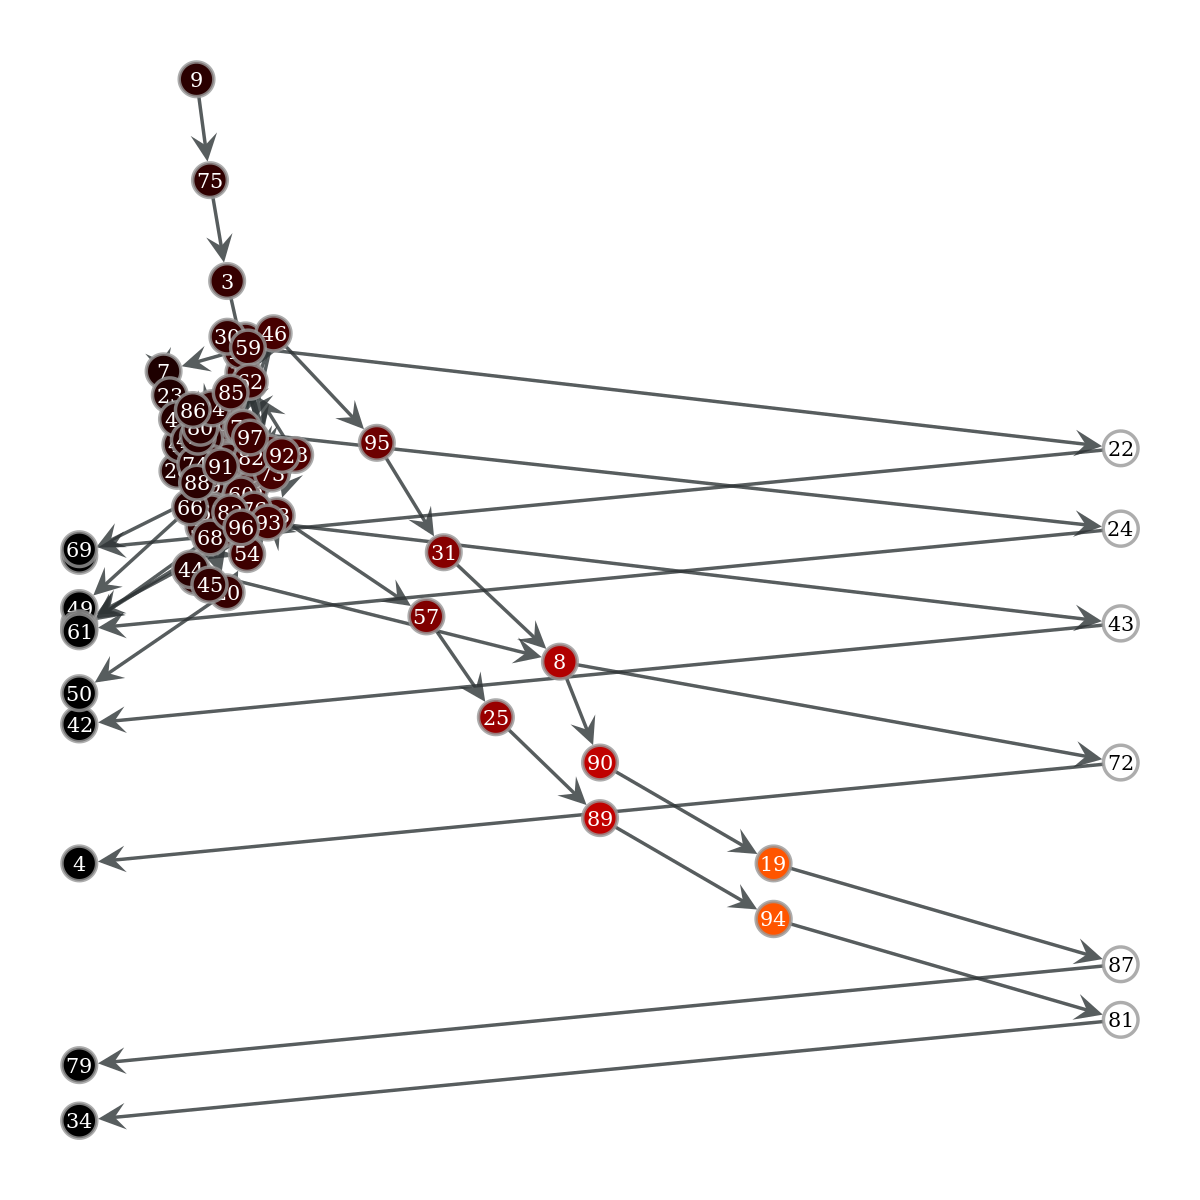
\includegraphics[scale=0.2]{frenchcloseness.png}
	\caption{ }
	\label{fig:frcc}
\end{subfigure}
\caption{Graphs with (a) betweenness and (b) closeness centrality values displayed on the $x$-axis based on the French numbered word graph. The $y$-axis being the trophic levels.}
\label{fig:frcentrality}
\end{figure}

Vertices with high betweenness will have many other vertices that must connect to it in order to reach other vertices within their sentence. As mentioned in previous language analysis, betweenness helps identify the key bridges in the sentences by finding the vertices which control the majority of the flow of data. Furthermore the betweenness coincides with the frequency. On the other hand there are vertices such as vertex 78 (``roi") and vertex 38 (``fois") who have a betweenness value of $6.73$ and $5.54$ (see Table \ref{table:frenchtablebc})respectively but only a count of 2 and 1. By further analysis, the reason they have high betweenness, is that they are used with a predecessor and successor of higher betweenness value, i.e. ``un roi et" and ``une fois un". Consequently causing its own betweenness value to be inflated because "un", "et" and "une" must pass through ``roi" or ``fois" to complete their word pathing. Therefore, if vertices have a low count but are connected to other vertices of high betweenness, then their values will relatively increased.

As discovered in the German analysis, closeness centrality identifies the vertices most likely divide the graph from their directed path, i.e. the words most likely to isolate the remaining sentence. Otherwise vertices are involved in a diverse range of sentences causing a high degree where the formation of vertex conglomerates can be seen (see Figure \ref{fig:frcc} where a clustering of vertices is shown in the upper left quadrant). Studying the graph in Figure \ref{fig:frcc}, French words have more vertices with a variety of high closeness values. The graph shows clearly that vertices of high closeness would cause isolation for further vertices along its path. According to the visualisations, French is the most unique language out of the three languages seen so far as there is a higher number of clear divisions in the closeness values.

\begin{figure}[!htb]
\centering
\begin{subfigure}{.45\textwidth}
	\hspace{-1cm} 
	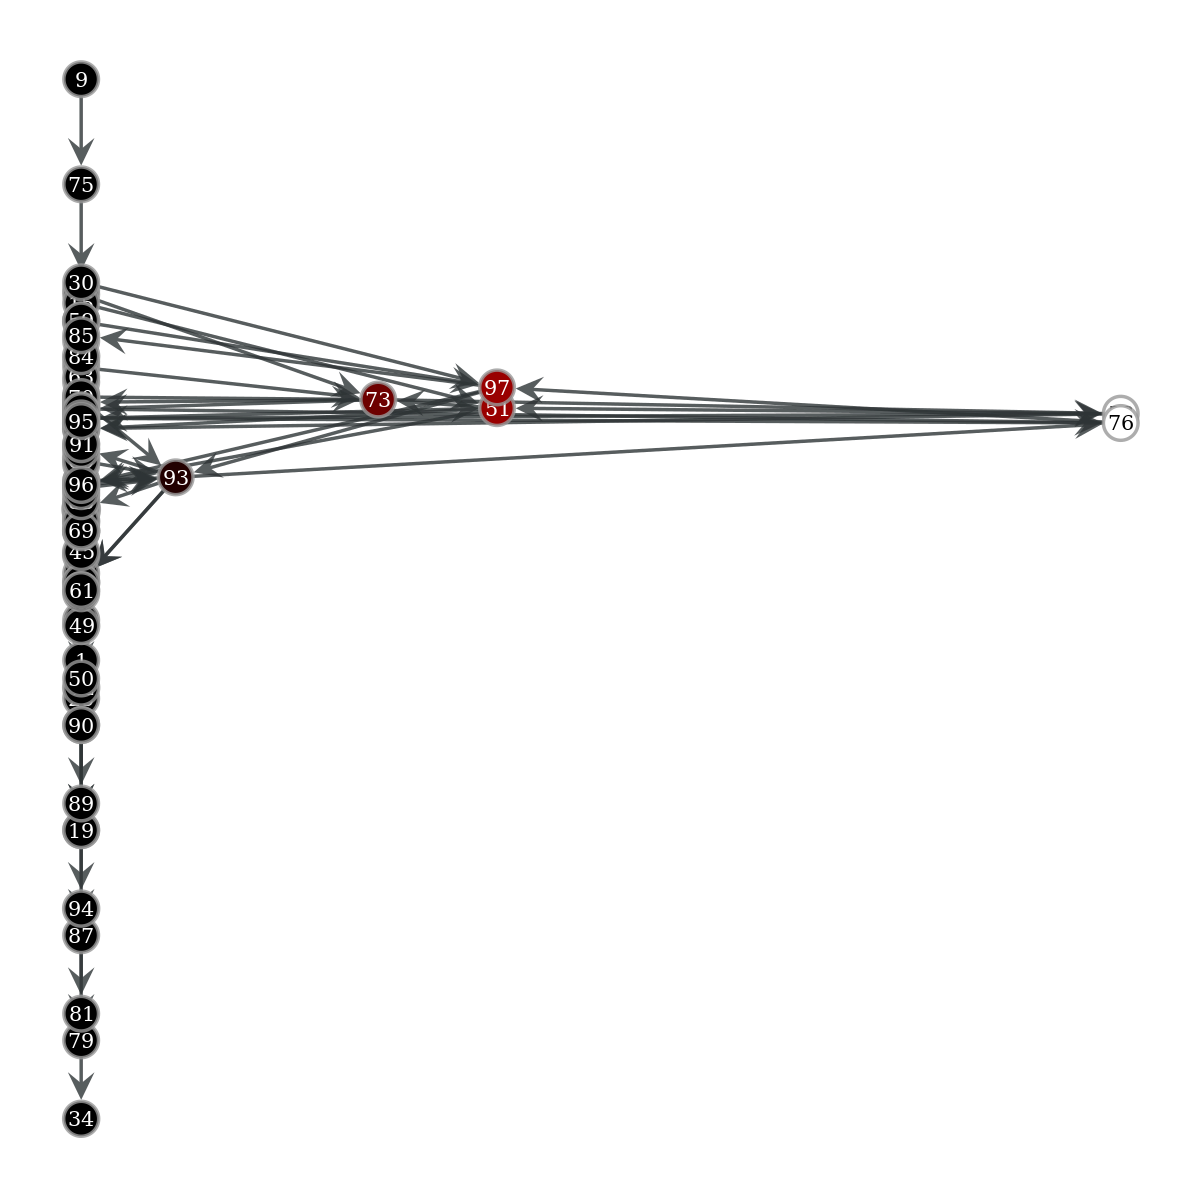
\includegraphics[scale=0.2]{frenchlocalclustering.png}
	\caption{}
	\label{fig:frlc}
\end{subfigure}
\hfill
\begin{subfigure}{.45\textwidth}
	\hspace{-1cm} 
	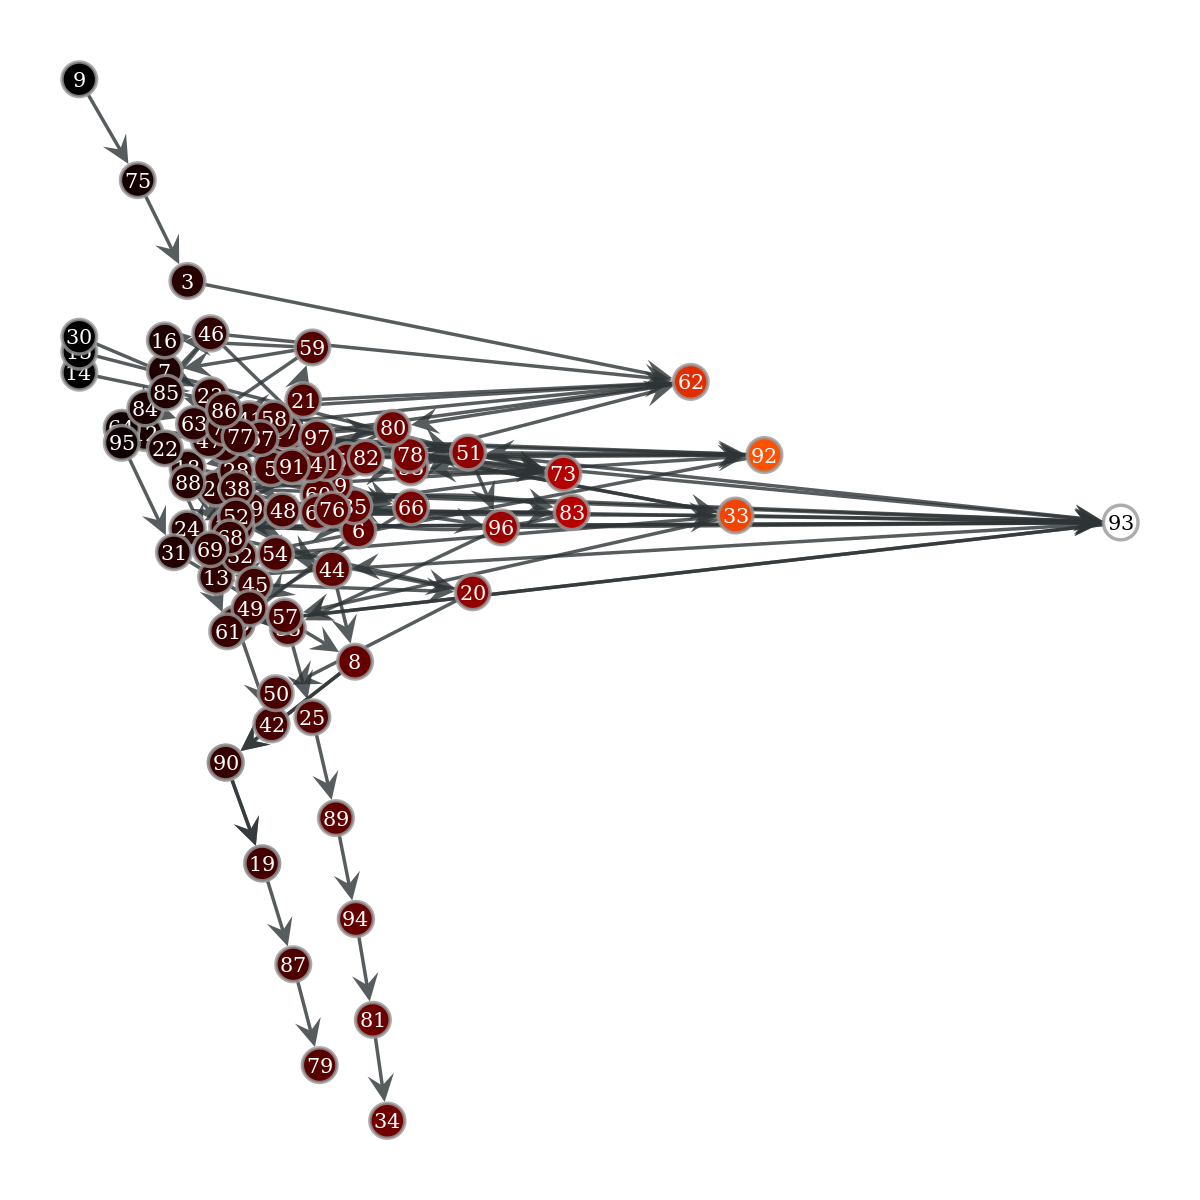
\includegraphics[scale=0.2]{frenchpagerank.png}
	\caption{}
	\label{fig:frpr}
\end{subfigure}
\caption{Graphs displaying the (a) local clustering and (b) page rank on the $x$-axis instead of the centrality values whilst keeping their $y$ positions.}
\label{fig:frother}
\end{figure}

Finally the local clustering coefficients and page rank. Only two vertices have a local clustering coefficient of $10$ which are vertex 53 ``le" and vertex 76 ``reine" (see Figure \ref{fig:frlc} and Table \ref{table:frenchtablelc}). In the context of French, nothing particular can be derived. However when studying the graphs of local clustering in various languages, the vertices with a local clustering value are never an start or end to a branch.

Page ranks for the French story corpus measures the influence the vertices have on one another other than for their immediate neighbours. This is why vertex 46 ``il" has a low page rank value of $1.26$ as it is located at the start of the sentence so does not have enough unique vertices encompassing it to be influential.

In conclusion, French has similar results in comparison to English and German which makes sense as they are a part of the same language family. So to see a different perspective, the study of other language families are undertaken such as the Japonic language family.

\section{Japonic}
The Japonic language family is the protolanguage for Japanese and Ryūkyūan languages \cite{vovin2017origins} so it is a relatively small language family compared to other language families. Translating the corpus into Japanese gives us a new dataset to use for graph property analysis which will be studied in comparison to the previous language family.
\subsection{Japanese}
To give a larger variety of languages, Japanese is studied as it uses vastly different grammar compared to the languages seen so far. Japanese has only five lexical word classes which includes nouns, verbal nouns, nominal adjectives, verbs and adjectives. The order in which the words are structured is different to Indo-European languages since Japanese uses SOV (Subject-Object-Verb) compared to languages like German and English which uses SVO (Subject-Verb-Object). Furthermore Japanese does not rely heavily on grammatical number or gender and is more focused on their system of honorifics which indicates the speaker, listener or person of reference. Therefore, even if Japanese contains words borrowed from other languages (these are referred to as \emph{loanwords} \cite{miura1979influence}), their grammar is vastly different. 

We follow the same process as before and input the Japanese Story corpus into my program to produce the basic graphs. For simplicity, we show the numbered version of the word graph (see Figure \ref{fig:jpgraph}) with the words they correspond to in the full table of data (See Table \ref{app:}).

\begin{figure}[!htb]
\centering
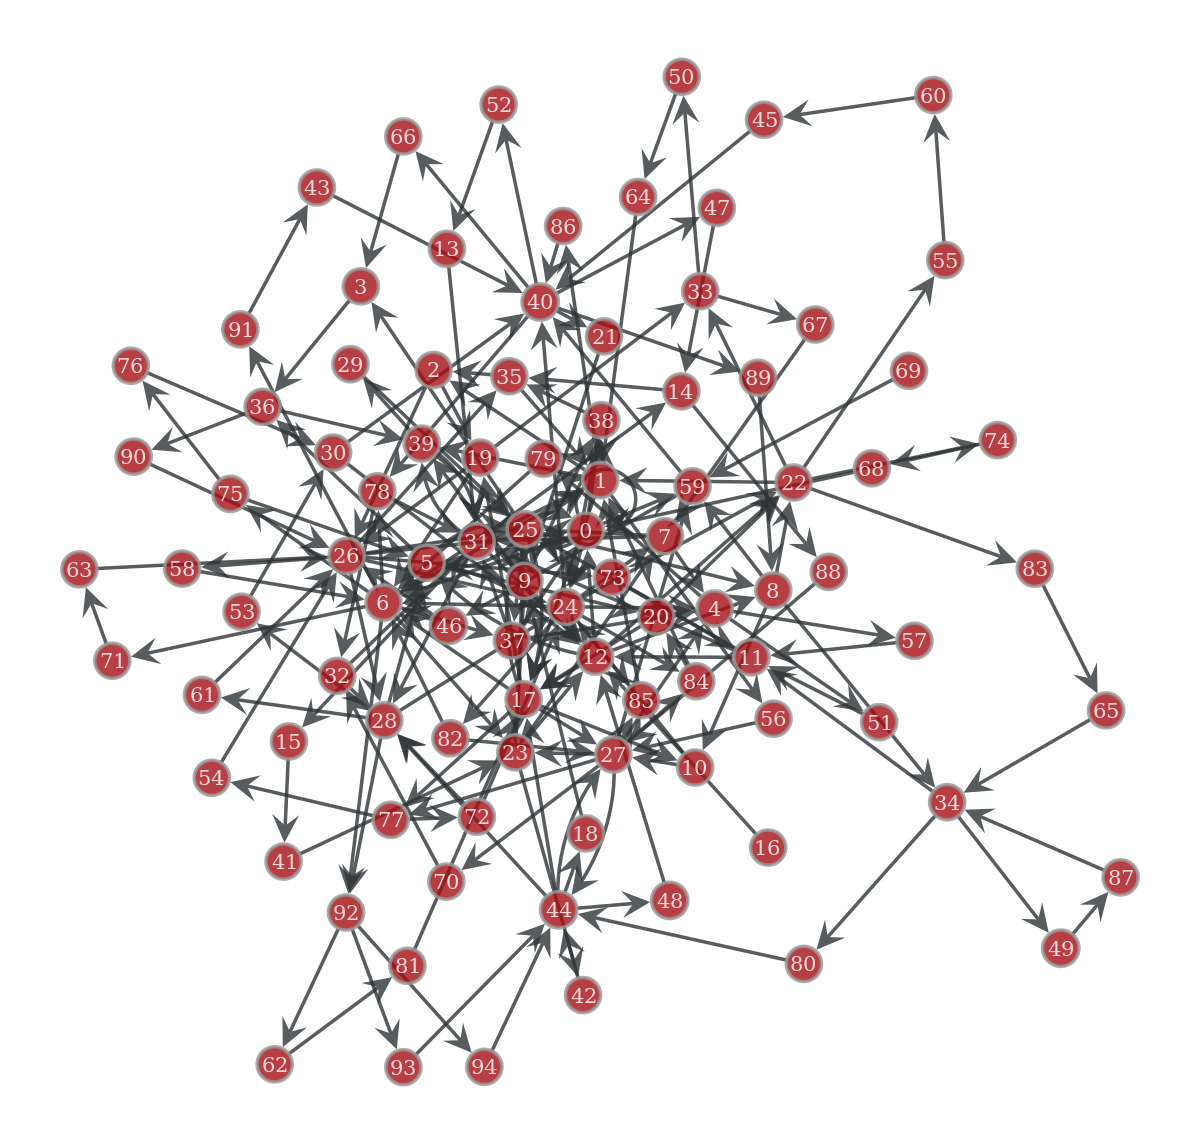
\includegraphics[scale=0.2]{japanesewordgraph.png}
\caption{The Japanese word graph generated from the Japanese translation of the story corpus.}
\label{fig:jpgraph}
\end{figure}

\begin{table}[!htb]
\centering
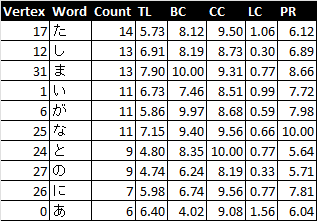
\includegraphics[scale=0.9]{japanesetabletop10.png}
\caption{Top 10 words with the highest frequency in the Japanese translation of the corpus. Shown in table format with other graphical properties. }
\label{table:japanesetop}
\end{table}

Out of the previous languages, the larger frequency of a words appearance was 9. With Japanese, there are 6 words with 11 or more appearances (see Table \ref{table:japanesetop}), largest being vertex 17 with 14 appearances. Vertex 17 represents a form of conjugation which means that their use depends on the inflections of its associated words. Generally vertex 17 is most commonly used to signify the past tense. So rather than having a separate word for different tenses, Japanese uses specific accompanying words which leads to their frequency being significantly higher. Additional examples such as vertex 12 who has a large frequency and its associated word is used to empathically add more information (an empathic and). Vertex 6 is a particle that means ``but" or indicates the sentence subject. Therefore, Japanese words have a heavy reliability on each other to define their overall meaning which is demonstrated by the many edges signifying these relationships.

\begin{table}[!htb]
\centering
\begin{subtable}{.45\textwidth}
	\centering
	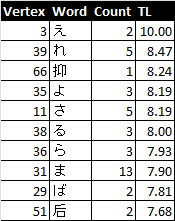
\includegraphics[scale=0.9]{jptabletctop.png}
	\caption{}
	\label{table:japanesentoptc}
\end{subtable}
\hfill
\begin{subtable}{.45\textwidth}
	\centering
	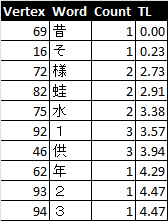
\includegraphics[scale=0.9]{jptabletcbot.png}
	\caption{}
	\label{table:japanesebottc}
\end{subtable}
\caption{Tables showing graph values ordered by (a) top 10 trophic levels and (b) bottom 10 trophic levels.}
\end{table}

Due to the graph having an increased amount of bidirectional edges such as the edge between vertex 25 and 5. As well as an increased amount of self loops, the trophic incoherence is very high in comparison to previous languages. Thus, the trophic coherence for the Japanese extract is only $0.04$. Caused by the ambiguity of hierarchical structure with bidirectional edges and self loops. An example of a self loop is vertex 0 which is part of the word ``everyday". The subsequent repetition of a word that creates a different meaning is known as \emph{reduplication}.

Unfortunately without a full understanding of the Japanese language, direct analysis of each word is difficult. This is because of the multitude of meanings each word has depending on the context. Therefore, the trophic levels can only provide a generic flow of text from lowest trophic levels (see Table \ref{table:japanesebottc}) as sentence starters to highest levels (see Table \ref{table:japanesetoptc})  as sentence enders.

\begin{table}[!htb]
\centering
\begin{subtable}{.2\textwidth}
	\centering
	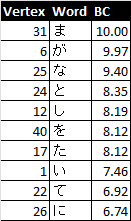
\includegraphics[scale=0.9]{japanesetablebc.png}
	\caption{}
	\label{table:japanesetablebc}
\end{subtable}
\hfill
\begin{subtable}{.2\textwidth}
	\centering
	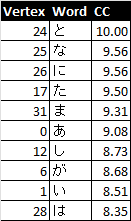
\includegraphics[scale=0.9]{japanesetablecc.png}
	\caption{}
	\label{table:japanesetablecc}
\end{subtable}
\hfill
\begin{subtable}{.2\textwidth}
	\centering
	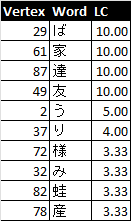
\includegraphics[scale=0.9]{japanesetablelc.png}
	\caption{}
	\label{table:japanesetablelc}
\end{subtable}
\hfill
\begin{subtable}{.2\textwidth}
	\centering
	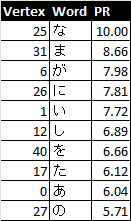
\includegraphics[scale=0.9]{japanesetablepr.png}
	\caption{}
	\label{table:japanesetablepr}
\end{subtable}
\caption{Partial extracts of the Japanese table data ordered by their (a) betweenness centrality values, (b) closeness centrality values, (c) local clustering coefficients and (d) page ranks.}
\label{table:japanesedatar}
\end{table}

As with previous languages, Tables \ref{table:japanesedatar} (a)-(d) are ordered extracts from the main table in Appendix \ref{app:}.

\begin{figure}[!htb]
\centering
\begin{subfigure}{.45\textwidth}
	\hspace{-1cm} 
	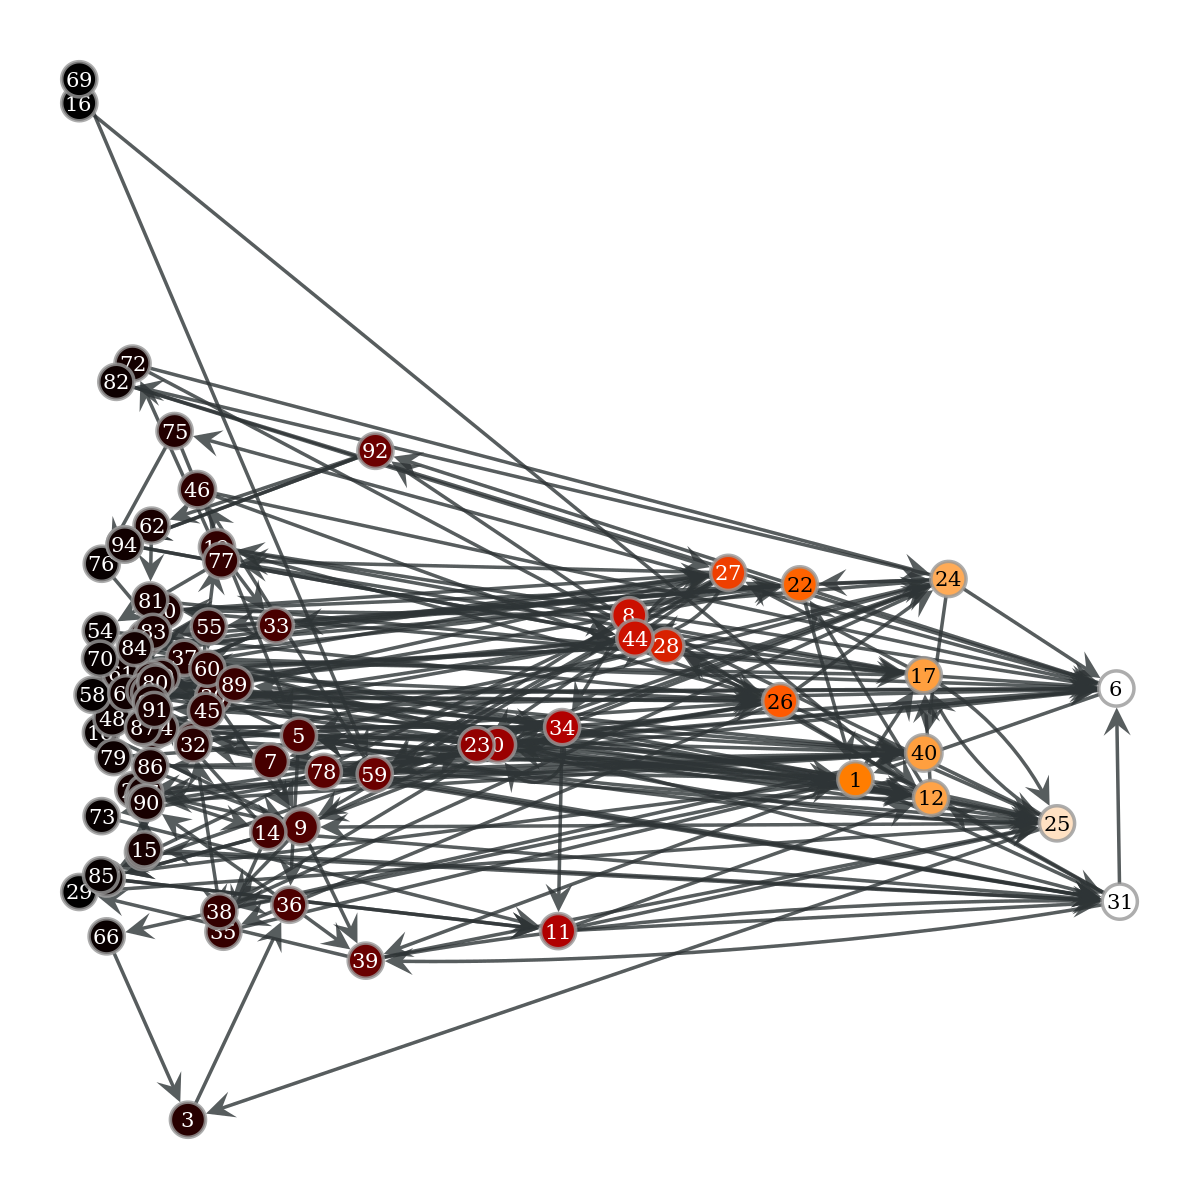
\includegraphics[scale=0.2]{japanesebetweenness.png}
	\caption{}
	\label{fig:jpbc}
\end{subfigure}
\hfill
\begin{subfigure}{.45\textwidth}
	\hspace{-1cm} 
	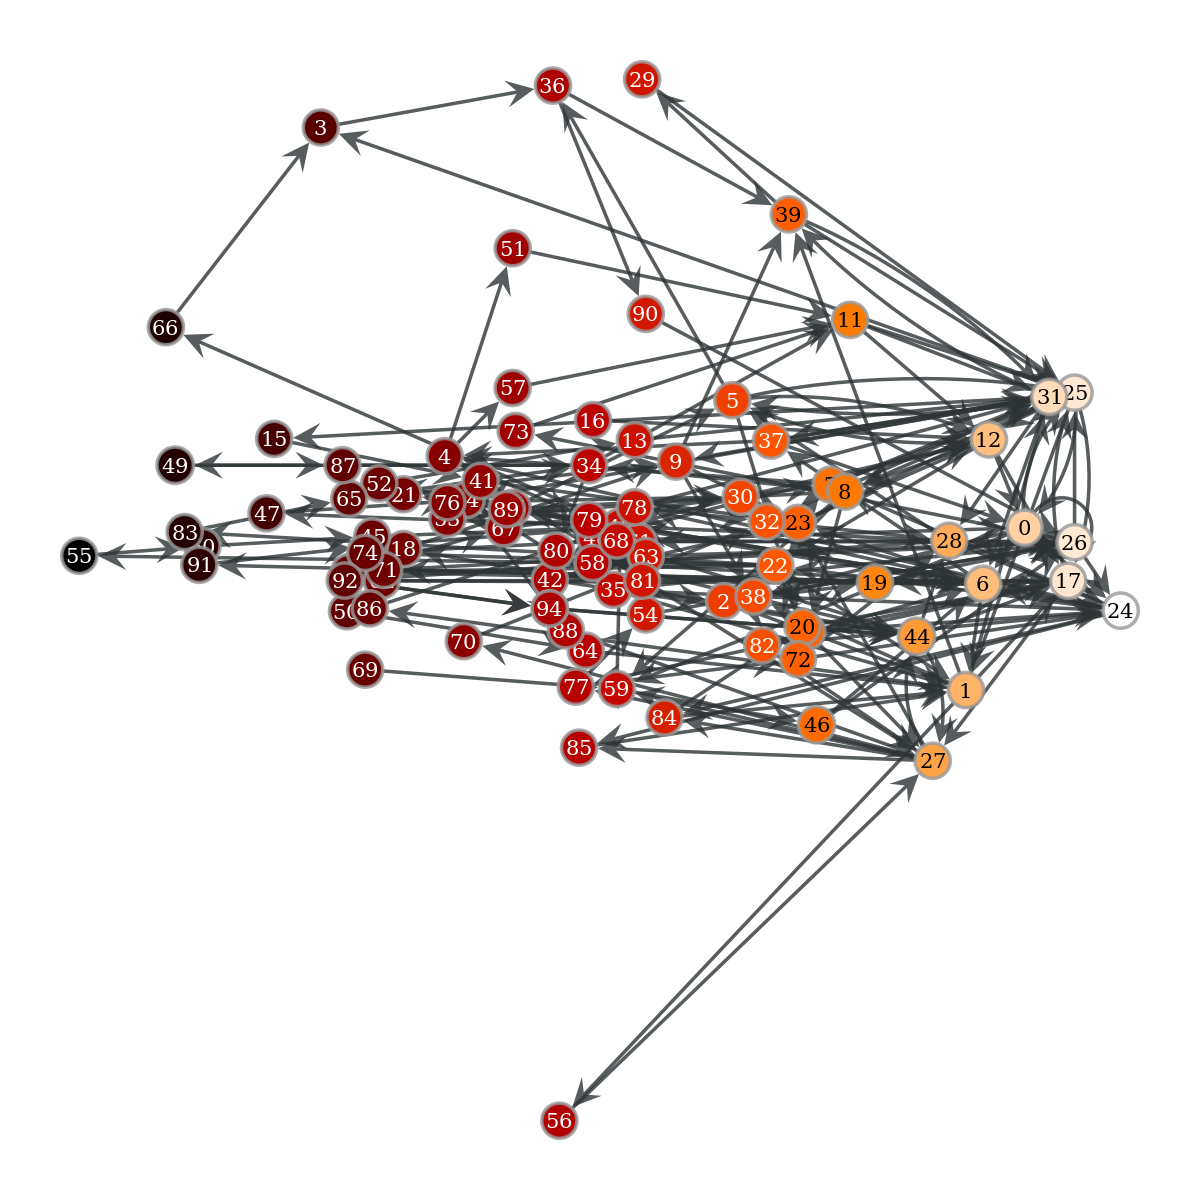
\includegraphics[scale=0.2]{japanesecloseness.png}
	\caption{ }
	\label{fig:jpcc}
\end{subfigure}
\caption{Positions of the Japanese numbered graph but with trophic levels on the $y$-axis and (a) betweenness or (b) closeness on the $x$-axis.}
\label{fig:jpcentrality}
\end{figure}

The graphs in the centrality Figure \ref{fig:jpcentrality} shows that the words are more evenly distributed unlike the Indo-European languages. Which correlates to the importance of the Japanese characters nature of being reliant on one another for their meaning and demonstrates the complexities of the language visually. The basic correlations from other languages still hold here. Although further detail cannot be determined by the visualisation other than importance.

Japanese's closeness centrality values also has a larger average compared to the Indo-European languages. Instead of looking at the vertices in relation to the whole graph, closeness focusses on the closer clusters. Hence provides a similar shape betweenness but shifted right to emphasise the zooming in on the vertices. There are no vertices that stand out so no correlations can be easily derived.

Therefore only a general correlation can be demonstrated through the centrality graphs. Clearer results can be gathered with Japanese fluency.

\begin{figure}[!htb]
\centering
\begin{subfigure}{.45\textwidth}
	\hspace{-1cm} 
	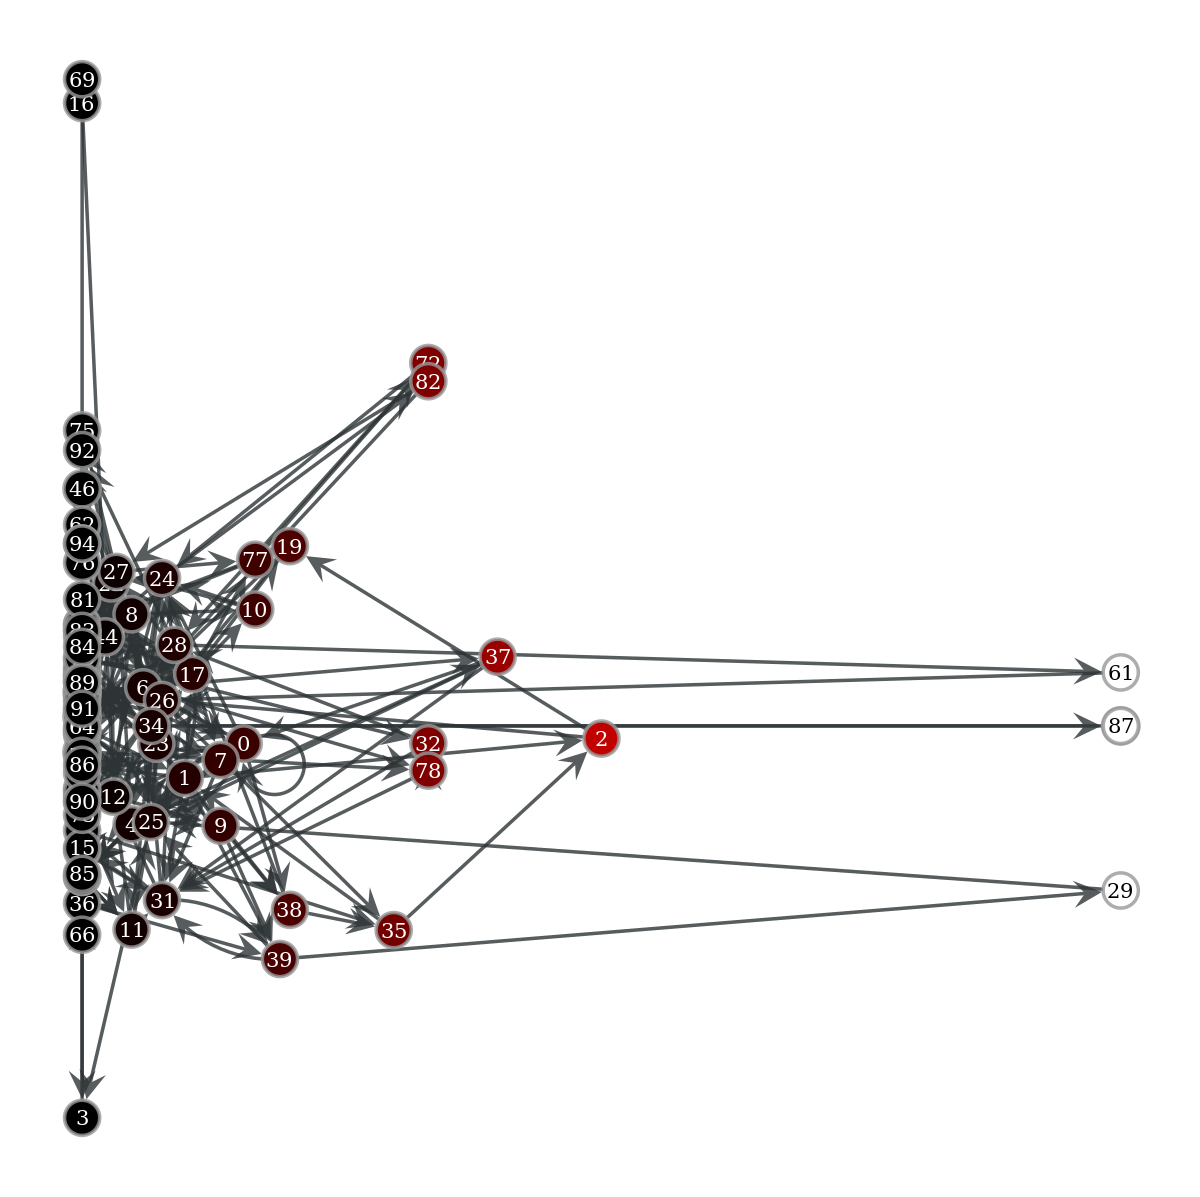
\includegraphics[scale=0.2]{japaneselocalclustering.png}
	\caption{Displays the local clustering coefficient against the trophic levels.}
	\label{fig:jplc}
\end{subfigure}
\hfill
\begin{subfigure}{.45\textwidth}
	\hspace{-1cm} 
	\includegraphics[scale=0.2]{japanesepagerank.png}
	\caption{Displays the page rank against the trophic levels.}
	\label{fig:jppr}
\end{subfigure}
\caption{The $x$-axis showing (a) local clustering and (b) page rank instead of the centrality values. The $y$ values remain.}
\label{fig:jpother}
\end{figure}

Local clustering coefficients (see Figure \ref{fig:jplc}) measures how close the vertex is part of a unique directed triangle, i.e. a directed 3 cycle. The vertices 29, 87 and 61 are vertices who are involved in such triangles where they each have a unique in and out edge to other vertices. Lower values means they are less likely to be involved in unique triangles. Thus local clustering can identify certain triples in the Japanese texts that would have unique meanings. 

Page rank identifies the vertices who have an influence to other vertices nearby but not immediate neighbours like what closeness does. However nothing further can be correlated based on this graph (see Figure \ref{fig:jppr}).

In conclusion the way the Japanese story corpus is split into the database (character by character), only general correlations can be determined based upon the graphs and their properties. Stronger links as to what exact words have importance cannot be obtained here without the full understanding of the language. On the other hand, we see that in general the graphs are different to the ones based on the Indo-European languages which demonstrates the languages differences. To see this further we analyse another language and its language family.

\section{Sino-Tibetan}
Sino-Tibetan is the final language family in which we analyse and contains over 400 languages. Two groups of languages that are successors of this family are the Tibeto-Burman language group and Chinese language group. Focus on the Chinese language will be taken to translate the story corpus into. Mandarin Chinese is chosen here since it is the 2nd most spoken language after English.

\subsection{Chinese}
The main branches of Chinese are Mandarin or Cantonese with Mandarin considered to be the standard and is the official language of China. Mandarin is also the language in which the corpus was translated into but will refer to this as Chinese for simplicity. Chinese has a SVO (subject-verb-object) sentence structure like with English. However the language is made up of syllables \cite{ross2017modern} rather than words. Syllables come with 3 parts, an initial consonant, the tone, and a final. These parts determines the meaning to each syllable and instead of writing their unique characters, they can be written using Pinyin. Pinyin is the standard system for romanised spelling and a useful tool in learning Chinese and their pronunciations. A simple word like ``hello" is ``nǐ hǎo" in Pinyin where ``n" and ``h" are initials, ``i" and ``ao" are finals and the accents on the letters ``i" and ``a" are the tone for the syllables. The tone matches the pitch of the syllable and leads to different meanings for the each word. Although each syllable in Chinese has its own definitions, they can be combined to form a different word. E.g. In Pinyin, ``dì" means earth but "dì tú" means map.

Similarly to Japanese, Chinese has very few inflectional characters and utilises other particles to accompany the syllables so various verbal aspects can be expressed. Another similarity is the use of reduplication where a syllable is repeated to give a different meaning. Parts of speech for Chinese is split into two major categories, the \emph{function} words and the \emph{content} words. The function words contains nouns, pronouns, verbs, auxiliary verbs, adjectives, number words, measure words, interjections and onomatopoeias. Function words contain conjunctions, prepositions and particles. Furthermore, each subgroup mentioned can have further branches dependent on the context that they are used in. For example, nouns can be proper nouns, location nouns, place nouns and time nouns in the Chinese language.

Therefore Chinese contains a larger amount of unique syllables compared to the words in the English language. Also syllables have a reliability factor and depends on the context of use (like when studying Japanese). Keeping this in mind, we generate and analyse the graphs beginning with seeing the basic word graph generated for the Chinese translation of the story corpus, seen in Figure \ref{cngraph} (shown with integer labelling to reference each word of the entire table, Table ?? in the Appendix).

\begin{figure}[!htb]
\centering
\includegraphics[scale=0.2]{chinesewordgraph.png}
\caption{The Chinese word graph generated from the Chinese translation of the story corpus.}
\label{fig:cngraph}
\end{figure}

\begin{table}[!htb]
\centering
\includegraphics[scale=0.9]{chinesetabletop10.png}
\caption{Top 10 words with the highest frequency in the Chinese translation of the corpus. Shown in table format with other graphical properties. }
\label{table:chinesetop}
\end{table}

The syllables with the highest count (see Table \ref{table:chinesetop}) is vertex 90 which is ``de" in Pinyin. This is a particle so has a grammatical meaning with different functions to denote possession. Also can be accompanied by other parts of speech. Other syllables with high counts include vertex 71, ``yǒu", vertex 5, ``gè" and vertex 0, ``yī". These vertices all have various meanings depending on their use, ``yǒu" can mean ``have", ``is" and ``are", ``gè" can mean ``this", ``that", the party of a specific size or a classifier for people or objects. Vertex 0, ``yī", can mean ``a" or is a part of a number like ``1" in the English language. Therefore the syllables with a high count represents the words of varied meanings which are important in the sentence structure or identifiers for words with different genders.

\begin{table}[!htb]
\centering
\begin{subtable}{.45\textwidth}
	\centering
	\includegraphics[scale=0.9]{cntabletctop.png}
	\caption{}
	\label{table:chinesetoptc}
\end{subtable}
\hfill
\begin{subtable}{.45\textwidth}
	\centering
	\includegraphics[scale=0.9]{cntabletcbot.png}
	\caption{}
	\label{table:chinesebottc}
\end{subtable}
\caption{Tables to show the (a) top 10 trophic level and (b) the bottom 10 along with other relative data.}
\end{table}

An increased amount of reduplications and bidirectional edges appear in the Chinese graph. Like before with the Japanese data, trophic levels do not demonstrate a clear visual hierarchy. Meaning that the trophic coherence is low and is calculated to be $0.09$ based on the Chinese translation of the story corpus. Therefore average positions of each syllable within a sentence can still be represented but with minor flexibility. The trophic levels go from low to high in relation to the sentence flow with Table \ref{table:chinesetoptc} showing the top 10 syllables nearer the start of a sentence and Table \ref{table:chinesebottc} showing the top 10 syllables for the end. Grammatically correct can be seen by unique downward paths in the graph visualisations such as the path from vertex 19 to vertex 61 (see Figure \ref{fig:cncentrality} or \ref{fig:cnother}).

\begin{table}[!htb]
\centering
\begin{subtable}{.2\textwidth}
	\centering
	\includegraphics[scale=0.9]{chinesetablebc.png}
	\caption{}
	\label{table:chinesetablebc}
\end{subtable}
\hfill
\begin{subtable}{.2\textwidth}
	\centering
	\includegraphics[scale=0.9]{chinesetablecc.png}
	\caption{}
	\label{table:chinesetablecc}
\end{subtable}
\hfill
\begin{subtable}{.2\textwidth}
	\centering
	\includegraphics[scale=0.9]{chinesetablelc.png}
	\caption{}
	\label{table:chinesetablelc}
\end{subtable}
\hfill
\begin{subtable}{.2\textwidth}
	\centering
	\includegraphics[scale=0.9]{chinesetablepr.png}
	\caption{}
	\label{table:chinesetablepr}
\end{subtable}
\caption{Partial extracts of the Chinese table data ordered by their (a) betweenness centrality values, (b) closeness centrality values, (c) local clustering coefficients and (d) page ranks.}
\end{table}

The top 10 syllables for each complex graph property is seen here where the full table is in Appendix \ref{app:}.

\begin{figure}[!htb]
\centering
\begin{subfigure}{.45\textwidth}
	\hspace{-1cm} 
	\includegraphics[scale=0.2]{chinesebetweenness.png}
	\caption{}
	\label{fig:cnbc}
\end{subfigure}
\hfill
\begin{subfigure}{.45\textwidth}
	\hspace{-1cm} 
	\includegraphics[scale=0.2]{chinesecloseness.png}
	\caption{ }
	\label{fig:cncc}
\end{subfigure}
\caption{Graphs showing (a) betweenness centrality and (b) closeness centrality values displayed on the x-axis based on the Chinese numbered word graph. The $y$-axis for their trophic levels.}
\label{fig:cncentrality}
\end{figure}

Betweenness centrality in the Chinese translation Story corpus (see figure \ref{fig:cnbc}) identified the syllables vertex 90 and vertex 10 (both are particles) to be of high importance. Re-emphasizing the fact that they are the syllables that act most like bridges and needed to derive further meaning. Hence betweenness relate closely to the counts of the syllables discussed earlier. The same correlation is achieved in previously discussed languages so we can conclude that this correlation of importance holds for the majority of languages.

As mentioned in the German analysis, closeness measures the importance of words directly around them. In other words, the vertices vital in the paths structure (controlling the flow of data). Therefore, demonstrated by Figure \ref{fig:cncentrality}, vertex 98 has the highest closeness as without this vertex, vertex 61 is isolated. Subsequently the predecessors of vertex 98 have higher closeness. However there are no other vertices with high closeness since other syllables hold connections to various unique vertices. Thus inferring that these syllables of high degree have multiple meanings rather than the unique meaning of vertex 98s section of the path.

\begin{figure}[!htb]
\centering
\begin{subfigure}{.45\textwidth}
	\hspace{-1cm} 
	\includegraphics[scale=0.2]{chineselocalclustering.png}
	\caption{}
	\label{fig:cnlc}
\end{subfigure}
\hfill
\begin{subfigure}{.45\textwidth}
	\hspace{-1cm} 
	\includegraphics[scale=0.2]{chinesepagerank.png}
	\caption{}
	\label{fig:cnpr}
\end{subfigure}
\caption{Displays the (a) local clustering and (b) page rank on the $x$-axis instead of the centrality values. The $y$ values are unaffected.}
\label{fig:cnother}
\end{figure}

By taking what we found in the Japanese graphs, we now know that the local clustering coefficient identifies vertices involved in unique directed 3-cycles. For example, vertex 22 is uniquely part of the directed 3-cycle, vertex 0 $\rightarrow$ 22 $\rightarrow$ 71 $\rightarrow$ 0 where vertex 22 is seen as the pinnacle of the cycle because vertices 22 and 71 hold other edge connections within the graph seen in Figure \ref{fig:cnlc}. The same applies to vertex 94 as it is involved in its own directed 3-cycle. So local clustering does not identify the vertices of high importance but rather certain triples within the corpus.

The page rank (see Figure \ref{fig:cnpr}) identifies the vertices with influence to vertices other than their immediate neighbours. Evidently vertices with high betweenness will also have a high page rank as they are more commonly used in the corpus. Similar results have been seen with other languages for page ranks so evidently, page rank and betweenness values are close in the context of lexical analysis.

